\chapter{STAT 256}
\section{Lecture Zero: Causal Inference vs Association}{Amanda Coston}

\subsection{Causal Inference on the Effect of Red Wine on Health}\label{sec:intro}

\subsection{Is red wine good for heart health?}
For many years consensus held that red wine improved cardiovascular health. The evidence behind this was largely from studies on people of drinking age that compared the health outcomes of those who self-reported that they drank wine to those who self-reported that they did not. Findings under such a design showed that people who drink  red wine have better cardiovascular outcomes than those who don't drink alcohol.

What are potential problems with this study design? You may be thinking that people who drink wine systematically differ from those who don't in ways that matter for health outcomes. In fact, sociologist Kaye Middleton Fillmore showed that the statistical significance of these findings hinged on the inclusion of \emph{previous} drinkers in the ``non-drinkers" category. That is, some people who said they did not drink red wine previously drank alcohol. Problematically, a common reason these people gave up alcohol was poor health. Therefore the definition of  ``non-drinkers" selected for people who had poorer health outcomes. Fillmore showed that redefining ``non-drinkers" to be ``never-drinkers" eliminated any supposed advantage of drinking wine.

The debate here was one of causal inference -- looking at the cause and effect of red wine on health.

For more details, see \cite{fillmore2007moderate}.

\subsection{Syllabus}

See course syllabi here: \href{https://stat156.berkeley.edu/fall-2024/syllabus.html}{https://stat156.berkeley.edu/fall-2024/syllabus.html}.

\subsection{Association vs Causation}

Association is the focus of much of statistics but in causal inference our focus is, of course, on causation! As a starting point, we will today consider common measures of association and discuss why they may not capture causation. In the next lecture we will see causal analogues of these measures.
aaa
We first consider the setting where the outcome $Y$ and treatment $Z$ are both binary. 

\begin{definition}[Risk Difference]
    The associative risk difference (RD) is $E[Y \mid Z = 1] - E[Y \mid Z = 0]$.
\end{definition}


\begin{definition}[Risk Ratio]
    The associative risk ratio (RR) is $P[Y =1 \mid Z = 1]/P[Y =1 \mid Z = 0]$.
\end{definition}

\begin{definition}[Odds Ratio]
    The associative odds ratio (OR) is $\frac{P[Y =1 \mid Z = 1]}{P[Y =0 \mid Z = 1]}/\frac{P[Y=1 \mid Z = 0]}{P[Y=0 \mid Z = 0]}$.
\end{definition}

Which measure one chooses depends on their particular setting -- what question they are interested in and what data they have available (odds ratios can be estimated in with outcome-dependent sampling whereas the risk difference and risk ratio generally cannot). The measures are related to each other as follows:

\begin{enumerate}
    \item $Z \perp Y  \Longleftrightarrow \mathrm{RD} = 0 \Longleftrightarrow \mathrm{RR} = 1 \Longleftrightarrow \mathrm{OR} = 1$
    \item $\mathrm{RD} > 0 \Longleftrightarrow \mathrm{RR} > 1 \Longleftrightarrow \mathrm{OR} > 1$ assuming all conditional probabilities are non-zero.
    \item $\mathrm{RR} \approx \mathrm{OR}$ when $P(Y=1)$ is small.
\end{enumerate}

Next we consider measures of association that can accommodate non-binary outcomes. 

\subsection{Correlation and linear regression}
Suppose we are now interested in the outcome blood pressure as a measure of cardiovascular health. A natural starting point is to model the relationship between blood pressure ($Y$) and whether one drinks red wine ($Z$) as 

\begin{align*}
    Y = \beta Z + \alpha + \epsilon
\end{align*}

where $E[\epsilon] = 0 $ and $E[\epsilon Z ] = 0$.

Recall that we can relate $\beta$ to the Pearson correlation coefficient $\rho$ as follows

\begin{align*}
    \beta = \rho \frac{\mathrm{var}(Z)}{\mathrm{var}(Y)}.
\end{align*}

The coefficient $\beta$ describes the change in $Y$ associated with whether one drinks red wine. More generally, the coefficient $\beta$ describes the change in $Y$ associated with one unit increase in $Z$.
Sometimes people refer to $\beta$ as the ``effect" of $Z$ on $Y$ but this is generally misleading (without further assumptions). We have simply modeled an associative relationship; we can't claim anything causal yet! Next time we will introduce a new language, potential outcomes, so that we can make causal claims.


\section{Lecture One: Potential Outcomes Framework}{Aryan Shafat, Frederik Stihler, Mika Lee (Revisions)}

\subsection{Review of last lecture}\label{sec:review}
Review of Risk Difference, Risk Ratio and Odds Ratio for setting where the outcome $Y$ and treatment $Z$ are both binary. (See lecture notes of Lecture 0 for details)

Explanation of the last equivalence in the following statement:
\begin{center}
$\mathrm{RD} > 0 \Longleftrightarrow \mathrm{RR} > 1 \Longleftrightarrow \mathrm{OR} > 1$ assuming all conditional probabilities are non-zero
\end{center}

We know that:

\begin{center}
    $\mathbb{P}[Y = 1 \mid Z = 1] + \mathbb{P}[Y = 0 \mid Z = 1] = 1$ and
    $\mathbb{P}[Y = 1 \mid Z = 0] +$ $\mathbb{P}[Y = 0 \mid Z = 0] = 1$. 
\end{center}    
    $\mathrm{RR} > 1$ implies that $\mathbb{P}[Y = 1 \mid Z = 1] > \mathbb{P}[Y = 1 \mid Z = 0]$, and hence $\mathbb{P}[Y = 0 \mid Z = 0] > \mathbb{P}[Y = 0 \mid Z = 1]$. This leads us to $\mathrm{OR} > 1$.

\subsection{Potential Outcome Framework}\label{sec:pof}

\subsubsection{Types of questions we are interested in}

\begin{enumerate}
    \item Does journaling reduce the risk of depression?
    \item Do personalized AI tutors improve a student's grade?
    \item Does smoking cigarettes cause cancer?
\end{enumerate}

We can summarize these questions in the following table: \par
\begin{center}
\begin{tabular}{ccc}
  \hline
  & \textbf{$Z$} & \textbf{$Y$} \\
  \hline
  1 & Journal & Depression \\
  \hline
  2 & AI tutor & Grade  \\
  \hline
  3 & Cigarettes & Cancer  \\
  \hline
\end{tabular}
\end{center}

For all the examples, we want to form a causal estimand using potential outcomes. The potential outcome framework was developed by \cite{neyman1923} in 1923 over one hundred years ago and later revitalized and repopularized by \cite{rubin1980} in 1980. 

\subsubsection{Potential Outcomes}

We are interested in potential (hypothetical) outcomes when we are thinking about causal questions.

\begin{definition}[Potential Outcome]
    The potential outcome Y is a function of a particular treatment value $Y(Z=z)$.
\end{definition}

E.g. $Y(Z=1) = Y(1)$ (the potential outcome under the intervention that assigns treatment) vs. $Y(Z=0) = Y(0)$ (the potential outcome under the intervention that assigns no treatment).

In our particular examples, these quantities are represented by the following hypothetical questions: \par

(1) Would someone have depression if they journalled $\approx Y(1)$ \\
(2) Would a  student get a particular grade if they had an AI tutor $\approx Y(1)$ \\
(3) Would someone get cancer if they smoked cigarettes $\approx Y(1)$

\subsubsection{Causal Estimands}

Next we define the causal versions of our measures of association (called  causal estimands).

\begin{definition}[Causal Risk Difference]
    The causal risk difference (on a population level) is $E[Y(1) - Y(0)]$.
\end{definition}

\begin{definition}[Causal Risk Ratio]
    The causal risk ratio is $\frac{E[Y(1)]}{E[Y(0)]} = \frac{P(Y(1) = 1)}{P(Y(0) = 1)}$.
\end{definition}

\begin{definition}[Causal Odds Ratio]
    The causal odds ratio is $\frac{P(Y(1) = 1)}{P(Y(1) = 0)}/\frac{P(Y(0) = 1)}{P(Y(0) = 0)} = \\ 
    \frac{E[Y(1)]}{E[1-Y(1)]}/\frac{E[Y(0)]}{E[1-Y(0)]}$.
\end{definition}

\subsubsection{Hidden Assumptions}

As mentioned, \cite{rubin1980} repopularized this framework by clarifying some important hidden assumptions:

\begin{assumption}[Consistency]
The treatment levels are well-defined (there are no other versions of the treatment).
\end{assumption}

\begin{assumption}[No Interference]
The treatment assigned to other units does not affect the potential outcomes for unit $i$ (no spillover).
\end{assumption}

These 2 assumptions are called \textbf{Stable Unit Treatment Value Assumption (SUTVA).}

For example, our 3rd question/example about cigarette smoking violates both assumptions.

The question isn't well-defined (does smoking entail  smoking 1 cigarette a day or smoking a whole pack a day) and thus violates Assumption 1.

It also violates Assumption 2, through non-smokers who might end up passively smoking by being around smokers.

\subsection{Causal Estimands}
Causal Effects are functions of potential outcomes. For example, the causal risk difference is essentially the 'average treatment effect'.

\begin{itemize}
    \item Unit 'i' has 2 potential outcomes: $Y_i$(1) and $Y_i$(0)
\end{itemize}

\begin{itemize}
    \item \textbf{Individualized treatment effect:} $Y_i$(1) - $Y_i$(0)
\end{itemize}

\textbf{Fundamental Problem of Causal Inference (1986 Holland):}
Never observe both potential outcomes.

\subsubsection{Add a time-element}
We could include a time element - write into our personal journal/smoke a cigarette/receive treatment one day and then go without treatment the next day, to see the 'causal effect' of the treatment.

However, the effect of the treatment might be long-lasting. Thus, one could 'experience'/observe their causal effects even on the days without treatment. Additionally, say for a time-period of 2 days, we actually end up having 4 potential outcomes:

\begin{itemize}
    \item $Y_{i, day 1}$(1) vs $Y_{i, day 1}$(0)
\end{itemize}

\begin{itemize}
    \item $Y_{i, day 2}$(1) vs $Y_{i, day 2}$(0)
\end{itemize}


Going back to the potential outcomes framework, we basically end up 'observing' one of the potential outcomes framework.

\begin{itemize}
    \item The factual/observed outcome is, $Y_i = 
\begin{cases}
Y_i(1) & \text{if } Z_i = 1 \\
Y_i(0) & \text{if } Z_i = 0
\end{cases}
$ 
\end{itemize}

Equivalently, 

$Y_i = Z_i*Y_i(1) + (1-Z_i)*Y_i(0)$

\begin{itemize}

\item The (unobserved) counterfactual, or missing potential outcome is given by:

$Y_i^{\text{mis}} = Z_i*Y_i(0) + (1-Z_i)*Y_i(1)$

\end{itemize}

\subsection{Simpson's Paradox}
Based on the class poll, we saw that the effect of the hint wasn't that strong. There was a confounding variable (row number) that was dampening the effect of the hint (since most of the hints were given to people in the rows at the back). This was attributed to \textbf{Simpson's Paradox}, which might have made it seem like the hints had an \textbf{effect reversal} (as if those who got the hints actually ended up doing worse on the poll).

This is mathematically shown as:
$\mathbb{P}(Y=1|Z=0) > \mathbb{P}(Y=1|Z=1)$. However, we can easily counter this by conditioning on the confounding variable (X):

\begin{center}
    $\mathbb{P}(Y=1|Z=0, X=x) < \mathbb{P}(Y=1|Z=1, X=x) \quad  \forall x \in X $
\end{center}

\subsubsection{Sources of the paradox:}
\begin{itemize}
    \item Confounding variables/factors
    \item Non-collapsibility
\end{itemize}

\section{Lecture Three: Randomized Experiments}{Daisy Wang \& Mika Lee (Revisions)}

\subsection{Last Lecture: Simpson's Paradox}
    Simpson's paradox is when the data may originally appear to have one trend, but not when grouped. In stats terms:
    
\begin{center}
    $\mathbb{E}[Y \mid Z=1] - \mathbb{E}[Y \mid Z=0] > 0$ 
\end{center}
but is actually 
\begin{center}
    $\mathbb{E}[Y \mid Z=1, X=x] - \mathbb{E}[Y \mid Z=0, X=x] <0$ 
\end{center} 
when we condition on the confounding variable X. This is caused by confounding and non-collapsibility.

    \textbf{Note on notation:} Potential outcomes $Y(Z=1) = Y(1)$ and in Hernan, $Y^{Z=1} = Y^1$

\subsection{Randomized Experiments}
    Why is randomization so powerful? 
    \begin{itemize}
        \item\textit{\textbf{Ignorable}} treatment assignment
        \item Groups are \textit{\textbf{exchangeable}}, in that groups could swap assignments and still have the same result
    \end{itemize}

\subsubsection{Exchangeability}
$\boldsymbol{\Pr{Y(1) = 1 \mid Z = 1}}= \Pr{Y(1) = 1 \mid Z = 0}$

$\Pr{Y(0) = 1 \mid Z = 1} = \Pr{Y(0) = 1 \mid Z = 0} =$
$ 
\boldsymbol{\Pr(Y = 1 \mid Z = 0)}$

where the two bolded equations are identifiable from the data. 

    Additionally $Y(Z) \perp Z$  $\forall  z = 0, 1$ which means treatment assignment is independent of potential outcome. In general, treatment assignment is exchangeable which implies ignorable which implied exogenous.

    In an \textbf{ideal random experiment}, association would be equal to causation:
\begin{center}$\mathbb{E}[Y \mid Z=1] = \mathbb{E}[Y(1)\mid Z=1]$ \end{center}
    Additionally:
\begin{center} Risk Difference $\mathbb{E}[Y \mid Z=1] - \mathbb{E}[Y\mid Z=0]$ = Causal Risk Difference $\mathbb{E}[Y(1)] - \mathbb{E}[Y(0)]$\end{center}
In tandem with the previous part about the independence of random treatment assignment, it is important to note that $Z \perp 
 Y(Z) \neq Z\perp Y$,  in which the relationship on the left side of the inequality contains random treatment assignment and the one on the right side references no treatment assignments.

    Finally a \textbf{randomized experiment} is where treatments are assigned in a known and probabilistic ("random") manner i.e. Bernoulli random experiments.

 \subsubsection{Completely Randomized Experiment}
    We denote those who get the treatment as $n_1$ , and those who get the control as $n_0 = n - n_1$. The treatment assignment is denoted as $\mathbb{Z}= (z_1, ... z_n)$.  Then the probability that $\Pr(\mathbb{Z}=z ) = \frac{1}{\binom{n}{n_1}}$ where $\mathbb{Z}$ is such that $\sum_{i=1}^{n} z_i = n_1$. Also keep in mind that $\mathbb{Y}(1)$ and $\mathbb{Y}(0)$ are fixed in this situation.

\subsubsection{Fisher (1935) Fisher's Sharp Null}
    $H_0: Y_i(1) = Y_i(0)$ for all $i = 1,...n$ where $\mathbb{Y} = \mathbb{Y}(1) = \mathbb{Y}(0)$ and the test statistic is $T(Z, \mathbb{Y})$. Here the $Z$ is random and $\mathbb{Y}$ is fixed. This is also known as Neyman's Null Hypothesis (Weak Null).
    
    Under the null, $\{T(z^1, \mathbb{Y})...T(z^{\binom{n}{n_1}}, \mathbb{Y}\}$ is uniform, representing the randomization distribution. Thus we can find the p-value:
    \begin{center} 
    $p = \frac{1}{\binom{n}{n_1}} \sum_{m=1}^{\binom{n}{n_1}} \mathbf{1}\{T(z^m,y) \geq T(Z, Y)\}$ 
    \end{center}
    We can also use the Monte Carlo method to approximate the p-value:
     \begin{center} 
     $\frac{1}{R} \sum_{r=1}^{R} \mathbb{1}\{T(z^r,y) \geq T(Z, Y)\}$ 
     \end{center}
     where $T(z^r,y) $ is a particular fixed value and $T(Z, Y)$ is an observed random variable.
     All of this is the \textbf{Fisher's randomization test}, aka \textbf{permutation test}.
     
 \subsubsection{Choices for the Test-Statistic}
 \paragraph{Difference-in-means statistic} 
$\hat{\tau} = \hat{\bar{Y}}(1) - \hat{\bar{Y}}(0)$ where $\hat{\bar{Y}}(1) = \frac{1}{n_1}\sum_{z_i=1}Y_i = \frac{1}{n_1}\sum_{i=1}z_iY_i $ 

\textbf{Note:} this statistic is easily ruined by outliers

\paragraph{Wilcoxon Rank Sum}
    Unlike the difference-in-means statistic, the Wilcoxon rank sum test statistic is robust to outliers. This is because it is defined as follows: 
    \begin{center} 
    $R_i:$ the rank of $Y_i = \#\{j: Y_j \leq Y_i\}$, and so the test statistic itself is  $W=\sum_{i=1}^{n}z_iR_i$ 
    \end{center}
    The test statistic is more broad and may miss distributional differences. It can also be viewed as the difference-in-means of the rank under treatment vs control. 

\paragraph{Kolmogorov-Smirnov Statistic}
The empirical CDF of treated units is $\hat{F_1}(y) = \frac{1}{n_1}\sum_{i=1}^n z_1 \mathbf{1}\{Y_i \leq y\}$  and the control is $\hat{F_0}(y) = \frac{1}{n_0}\sum_{i=1}^n (1-z_1) \mathbf{1}\{Y_i \leq y\}$. The test statistic is then
\begin{center} $D=\underset{y}{\max}|\hat{F_1}(y) - \hat{F_0}(y)|$ \end{center}






\section{Lecture Four: Continue on Randomized Experiments}{Yulin Zhang \& Aadya Agarwal}
\subsection{Last Lecture: Complete Randomized Experiments}
    \begin{itemize}
        \item Complete randomized experiment
        \begin{itemize}
            \item \textit{terms}: let $n$ denotes the total number of test units, $n_1$ denotes the number of units get treated, $n_0 = 1 - n_1$ denotes the number of units get control.
        \end{itemize}
        \item exchangability: $y(z) \perp z$, where $z$ denotes treatment, $y(z)$ denotes the outcome of the treatment.
        \item Fisher's sharp null
    \end{itemize}
    
\subsection{Neymanian estimation \& inference}

\subsubsection{Finite population counterfactual (potential) quantities}
Let $y_{i}(1)$ and $y_{i}(0)$ denote the potential outcomes of the $i$th unit under treatment and control. Define the \textit{individual casual effect} of the $i$th unit as $$\tau_{i} = y_{i}(1) - y_{i}(0)$$
\textbf{Theoretical population level statistics}:\\
$$\bar{y}(1)= \frac{1}{n}\sum_{i = 1}^{n}y_i(1)$$
$$\bar{y}(0)= \frac{1}{n}\sum_{i = 1}^{n}y_i(0)$$
$$S^{2}(1) = \frac{1}{n - 1}\sum_{i = 1}^{n}(y_i(1) - \bar{y}(1))^{2}$$
$$S^{2}(0) = \frac{1}{n - 1}\sum_{i = 1}^{n}(y_i(0) - \bar{y}(0))^{2}$$
$$S(1, 0) = \frac{1}{n - 1}\sum_{i = 1}^{n}(y_i(1) - \bar{y}(1))(y_i(0) - \bar{y}(0))$$
$$\tau = \frac{1}{n}\sum_{i = 1}^{n} \tau_{i} = \bar{y}(1) - \bar{y}(0)$$
$$S^{2}(\tau) = \frac{1}{n - 1}\sum_{i = 1}^{n}(\tau_{i} - \tau)^2$$

\textbf{Lemma}: $2S(1, 0) = S^{2}(1) + S^{2}(0) - S^{2}(\tau)$ \\

\textbf{In the data}:
$$\hat{\bar{y}}(1) = \frac{1}{n_1}\sum_{i = 1}^{n}z_{i}y_{i}$$
$$\hat{\bar{y}}(0) = \frac{1}{n_0}\sum_{i = 1}^{n}(1 - z_{i})y_{i}$$
$$\hat{S^{2}}(1) = \frac{1}{n_1 - 1}\sum_{i = 1}^{n}z_i(y_i - \hat{\bar{y}}(1))^{2}$$
$$\hat{S^{2}}(0) = \frac{1}{n_0 - 1}\sum_{i = 1}^{n}(1 - z_i)(y_i - \hat{\bar{y}}(0))^{2}$$
Note, since we could not observe $y_i(1)$ and $y_i(0)$ at the same time, no other theoretical statistics could be calculated at this point.

\subsubsection{Neyman (1993) theorm}
\begin{itemize}
    \item $\hat{\tau} = \hat{\bar{y}}(1) - \hat{\bar{y}}(0)$ satisfies:
    \begin{itemize}
        \item unbiasedness: $\mathbb{E}(\hat{\tau}) = \tau$
        \item has variance: $$\mathbb{V}(\hat{\tau}) = \frac{S^{2}(1)}{n_1} + \frac{S^{2}(0)}{n_0} - \frac{S^{2}(\tau)}{n} = \frac{n_0}{n_{1}n}S^{2}(1) + \frac{n_1}{n_{0}n}S^{2}(0) + \frac{2}{n}S(1, 0)$$
        \item Note in variance terms, $S^{2}(\tau)$ and $S(1, 0)$ are not identifiable from the data, this variance could not be calculated from the data directly.
    \end{itemize}
    \item Neyman's variance estimator: $$\hat{\mathbb{V}}(\hat{\tau}) = \frac{\hat{S^{2}}(1)}{n_1} + \frac{\hat{S^{2}}(0)}{n_0}$$
    \begin{itemize}
        \item Note: this is the usual variance estimator under the assumption that the population is infinite and random samples. However, this is not the case we have here: the population is finite and we do not have random samples (treatment and controls are usually mutually exclusive).
        \item In the paper, Neyman proved that $$\mathbb{E}(\hat{V}) - \mathbb{V}(\hat{\tau}) = \frac{S^{2}(\tau)}{n} \ge 0$$ where equality holds when $\tau_{i} = \tau $ $\forall i$. This shows that the estimator above is conservative for estimating the variance of $\hat{\tau}$. People call this a "minor miracle that the two mistakes cancel" (Freeman, Pisani \& Purues, 2006)
    \end{itemize}
    \item Regression analysis of the complete randomized experiment \\
    In OLS settings, we could get $(\hat{\alpha}, \hat{\beta}) = argmin_{a, b}\sum_{i = 1}^{n} (y_i - a - bz_i)^2$, where $\hat{\beta} = \hat{\tau}$
    \begin{itemize}
        \item Usual OLS variance: $\hat{\mathbb{V}}_{OLS}(\hat{\beta}) = \hat{\mathbb{V}}_{OLS}(\hat{\tau}) \approx \frac{\hat{S^{2}}(1)}{n_0} + \frac{\hat{S^{2}}(0)}{n_1}$, note this is not equal to the variance we want. 
        \item Eicker-Huber-White (EHW) Robust Variance Estimator: $\hat{\mathbb{V}}_{EWH}(\hat{\tau}) \approx \frac{\hat{S^{2}}(1)}{n_1} + \frac{\hat{S^{2}}(0)}{n_0}$
        \item HC2 variant of EHW $= \frac{\hat{S^{2}}(1)}{n_1} + \frac{\hat{S^{2}}(0)}{n_0}$
    \end{itemize}
\end{itemize}

\subsection{Stratified (Conditional) Random Experiments}
\subsubsection{A potential problem with completely randomized experiment}
Bias could be introduced if the different covariate strata have non-random treatments assigned. 
\begin{itemize}
    \item Let $x_i \in \{1..k\}$ denote a covariate that we are interested in.
    \item Covariate imbalance: bias would be introduced if the proportion of units in stratum $k$ are different across treatment and control groups. 
\end{itemize}
\subsubsection{Definition}
Let $n_{k, 1} = \# \{i: x_i = k, z_i = 1\}$, $n_{k, 0} = \# \{i: x_i = k, z_i = 0\}$. $n_{k} = \# \{i: x_i = k\}$ \\
Stratified random experiment (SRE) is to run $k$ independent complete random experiments (CRE) within k strata of discrete covariate $x$ for fixed $n_{k, 1}$, $n_{k, 0.}$ \\
We could view stratum as block, stratified randomization could also be called block randomization. \\
$$\tau_{k} = \frac{1}{n_k}\sum_{x_i = k} \tau_{i}$$
$$\tau = \frac{1}{n}\sum_{i = 1}^{n}\tau_i = \frac{1}{n}\sum_{k = 1}^{k}\sum_{x_i = k}\tau_i = \sum_{k = 1}^{k}\pi_{k}\tau_{k}, \pi_k = \frac{n_k}{n}$$
\textbf{Comparing SRE and CRE}:
\begin{itemize}
    \item Number of potential assignments: $SRE: \prod_{k = 1}^{k} \binom{n_k}{n_{k, 1}} < CRE: \binom{n}{n_1}$
    \item Propensity score (propensity of getting treatment): $e_k = \frac{n_{k, 1}}{n_k}$. For SRE, $e_k$ is fixed; for CRE, $e_k$ is random.
\end{itemize}

\subsubsection{Fisher Randomization Test}
$H_0: Y_i(0) = Y_i(1)$ for all i \\
Run Fisher Randomization test by permuting the treatment indicators within each strata X according to the fixed values of treatment assigned for each of those strata \\
This process is called the \textbf{Conditional Randomization Test or Conditional Permutation test}\\
\\
Test Statistic Choice: \\
\\
\textbf{1. Stratified Estimator\\}
$\hat{\tau}_s = \sum_{k=1}^{K} \pi_k \hat{\tau}_k$\\
\\
\textbf{2. Combined Wilcoxon-Rank Sum Statistic\\}
\\
$W_k$ : Wilcoxon rank-sum statistic in stratum k
\\$W_s = \sum_{k=1}^{k}C_k W_k$
\\$C_k = \frac{1}{n_k,_1 n_k,_0}$ OR $C_k = \frac{1}{n_k + 1}$\\
\\Note: Works well only if k is small
\\
\\\textbf{3. Aligned Rank Statistic (Hodges and Lehmann)} \\
\\$\tilde{Y}_i = Y_i - \bar{Y}_k$ where $Y_k = \frac{1}{n-k} \sum_{X_i = k} Y_k$ (stratum specific mean)
\\Let $\tilde{Y}_i$ be the rank of $\tilde{Y}_i$
\\ $\tilde{W} = \sum_{i=1} ^ {n} Z_i \tilde{R}_i$

\subsubsection{Neymanian Inference for SRE}

$\mathbb{E}[\hat{\tau}_k] - {\tau}_k = 0$
\\$\hat{\tau}_k$ has variance:
Var($\hat{\tau}_k$) = $\frac{S_k^2 (1)}{n_k,1} + \frac{S_k^2 (0)}{n_k,0} - \frac{S_k^2 (\tau)}{n_k} $
\\where $S_k^2(1), S_k^2(0), S_k^2(\tau)$ are the stratum specific analogs (stratum specific variance of potential outcomes and causal effects)
\\We can combine these to get a stratified estimator: $\hat{\tau}_s = \sum_{k=1}^{k} \pi_k \hat{\tau}_k$ where $\pi_k = \frac{n_k}{n}$ and 
\begin{itemize}
    \item $\mathbb{E}[\hat{\tau}_s] - \tau = 0$ (unbiased)
    \item has variance var($\hat{\tau}_s$) = $\sum_{k=1}^{k} \pi_k^2 var(\hat{\tau}_k)$
\end{itemize}
If $n_k,1 >= 2$ and $n_k,0 >= 2$, we can compute $\hat{S_k^2}(1)$, $\hat{S_k^2}(0)$
\\$\hat{V_s} = \sum_{k=1}^{k} \pi_k^2 (\frac{\hat{S_k^2}(1)}{n_k,1} + \frac{\hat{S_k^2}(0)}{n_k,0})$
\\$\hat{\tau_s} +- Z_{1-\frac{\alpha}{2}} \sqrt{\hat{V_s}}$
\\$H_o$ : $\tau = 0 $ \quad $\epsilon_s = \frac{\hat{\tau_s}}{\sqrt{\hat{V_s}}}$

\subsubsection{SRE vs CRE}
$e_k = e$ for all k, $\hat{\tau} = \hat{\tau_s}$
\\$var_{CRE} (\hat{\tau}) - var_{SRE} (\hat{\tau_s}) = \sum_{k=1}^{k}\frac{\pi_k}{n} (\sqrt{\frac{n_0}{n_1}} (\bar{Y_k}(1) - \bar{Y}(1)) + \sqrt{\frac{n_1}{n_0}} (\bar{Y_k}(0) - \bar{Y}(0)))^2 >= 0 $
\\$\hat{\tau_s}$ is generally more efficient (has lower variance) than $\hat{\tau}_{CRE}$

\subsubsection{Post-Stratification}

We've already run a CRE
\\$\textbf{n} = \{n_{k,1}, n_{k,0}\}_{k=1}^{K}$
\\$P_{CRE} (\textbf{Z}=z | \textbf{n}) = \frac{P(\textbf{Z}=z, \textbf{n})}{P(\textbf{n})}$ where $\textbf{Z} \epsilon R^n = \{Z_1, ...., Z_n\}$
\\= $\frac{1}{\pi_{k=1}^k \binom{n_k}{n_k,1}}$
\\How to choose k?
\\$k=5$ empirically is a good choice OR $k = \frac{n}{2}$ which is the 'matched pairs experiment'


\section{Lecture Five: Rerandomization and Regression Adjustment}{Inigo Artiagoitia \& Sai Kolasani}
\subsection{Last Lecture: Discrete Covariate}
    \begin{itemize}
        \item Design: Stratification
        \end{itemize}
    \begin{itemize}
        \item Analysis: Post-stratification
    \end{itemize}
\subsection{Completely randomized experiment}
$n$ total experimental units

$n_1$ units randomly assigned to the treatment group

$n_0$ units randomly assigned to the control group

number of ways to assign $n_1$ units to treatment out of $n$ total units in a CRE:
$$\mathbb{Z}\binom{n}{n_1}$$
\subsubsection{Rerandomization}

In rerandomization, we draw $Z$ from the CRE and accept it if and only if the covariates are balanced across treatment and control groups.

Also, we have covariates. For example:
\begin{itemize}
    \item $x_i \in \mathbb{R}^k$ (e.g., age)
    \item Outcome $y$ might be fitness, while treatment $z$ could be a health intervention
\end{itemize}

We want to ensure these covariates are balanced between our treatment and control groups. To check this, we calculate the difference in means of covariates:

\[
\hat{\tau}_x = \frac{1}{n_1} \sum_{i=1}^n z_i x_i - \frac{1}{n_0} \sum_{i=1}^n (1-z_i) x_i
\]

Under CRE, $E[\hat{\tau}_x] = 0$, meaning the covariates are perfectly balanced on average. However, in practice, we often see $\hat{\tau}_x \neq 0$.

The covariance of this difference is given by:

\[
\text{cov}(\hat{\tau}_x) = \frac{1}{n_1} S_x^2 + \frac{1}{n_0} S_x^2 
\]

\[
= \frac{n}{n_1 n_0} S_x^2
\]

\[
S_x^2 = \frac{1}{n-1} \sum_{i=1}^{n} x_i x_i^T
\]

\subsubsection{Mahalanobis Distance}

The following Mahalanobis distance measures the difference between the treatment and control groups:

\[
M = \hat{\tau}_x^T \, \text{cov}(\hat{\tau}_x)^{-1} \hat{\tau}_x 
\]

\[
= \hat{\tau}_x^T \left( \frac{n}{n_i n_0} S_x^2 \right)^{-1} \hat{\tau}_x 
\]

\subsubsection{Rerandomization Procedure}

For this, we:
\begin{enumerate}
    \item Draw $Z$ from CRE
    \item Accept if and only if $M \leq a$
\end{enumerate}

The value of 'a' determines how strict we are about balance:
\begin{itemize}
    \item $a = \infty \rightarrow$ We accept any randomization (equivalent to CRE)
    \item $a = 0 \rightarrow$ We only accept perfect balance (usually impossible)
    \item $a = 0.001 \rightarrow$ A good threshold used.
\end{itemize}

This procedure is invariant to linear transformations of covariates.

\subsubsection{Inference}

\begin{itemize}
    \item We use FRT that simulates $Z$ under the constraint $M \leq a$
    \item For $a = \infty$: $\varepsilon$ be a univariate standard normal RV, and $\hat{\tau} - \tau \stackrel{D}{\sim} \sqrt{\text{var}(\hat{\tau})} \varepsilon$
    \item For $a$ close to zero: $\hat{\tau} - \tau \stackrel{D}{\sim} \sqrt{\text{var}(\hat{\tau})(1-R^2)} \varepsilon$ where $R^2$ is the squared correlation between $\hat{\tau}$ and $\hat{\tau}_x$
\end{itemize}

\subsection{Regression Adjustment (analysis)}

FRT:
\begin{enumerate}
    \item Regress $Y_i \sim X_i \rightarrow \hat{Y}_i$. 
    $\hat{\varepsilon}_i = \hat{Y}_i - Y_i$: pseudo outcome for test statistic.
    \item Regress $Y_i \sim (Z_i, X_i) \rightarrow \hat{\beta}$ (coefficient of $Z_i$): Test statistic.
    \item Estimation $\tau$:
\end{enumerate}

\subsubsection{Fisher's ANCOVA (1925)}

\begin{enumerate}
    \item Run an OLS Regression: $Y_i \sim (1, z_i, x_i)$
    \item Use $\beta$ (coefficient of $Z$) as our estimator for $\tau = \hat{\tau}_F$
\end{enumerate}

However, this method was criticized because:
\begin{enumerate}
    \item Bias: $E[\hat{\tau}_F] - \tau \neq 0$
    \item $\text{Var}(\hat{\tau}_F) > \text{var}(\hat{\tau})$ for $n_1 \neq n_0$
    \item Standard errors from OLS are incorrect
\end{enumerate}

\subsubsection{Lin (2013) Improvements}

Lin proposed some improvements to address these issues:
\begin{enumerate}
    \item The bias $E[\hat{\tau}_F] - \tau$ is small for large $n$ and approaches 0 as $n \rightarrow \infty$
    \item Run an OLS Regression: $y_i \sim (1, z_i, x_i, x_i * z_i) \rightarrow \hat{\tau}_L$ (coefficient of $z$)
    \begin{itemize}
        \item $\hat{\tau}_L$ is more efficient than $\hat{\tau}_F$
    \end{itemize}
    \item EHW standard error gives conservative estimate for $\hat{\tau}_L$.
\end{enumerate}


\subsubsection{Difference-in-Differences}

\begin{itemize}
    \item A special case of covariate adjustment, where $X$ is the \textbf{lagged outcome before the treatment}.
    
    \item The estimator for the average treatment effect is given by:
    \[
    \hat{\tau}_{\text{DiD}} = \frac{1}{n_{1}} \sum_{i=1}^{n} z_i (Y_{i} - x_i) - \frac{1}{n_{0}} \sum_{i=1}^{n} (1 - z_i)(Y_{i} - x_i)
    \]
    where $n_{1}$ is the number of treated units and $n_{0}$ is the number of control units. 
    
    This expression represents the \textbf{difference in treated and control outcomes after adjusting for pre-treatment covariates (the lagged outcomes $x_i$).}
    
    \item This can be rewritten as:
    \[
    \hat{\tau}_{\text{DiD}} = \left( \hat{Y}(1) - \hat{Y}(0) \right) - \left( \hat{X}(1) - \hat{X}(0) \right)
    \]
    where:
    \begin{itemize}
        \item $\hat{Y}(1)$ and $\hat{Y}(0)$ are the mean outcomes for the treated and control groups, respectively.
        \item $\hat{X}(1)$ and $\hat{X}(0)$ are the mean pre-treatment covariates for the treated and control groups, respectively.
    \end{itemize}
    
    \item This estimator is \textbf{unbiased}, and the mean of the treatment and control groups are:
    \[
    \hat{g}(C1) = \frac{1}{n_{1}} \sum_{i=1}^{n} z_i g_i
    \]
    \[
    \hat{g}(C0) = \frac{1}{n_{0}} \sum_{i=1}^{n} (1 - z_i) g_i
    \]
    where $g_i = Y_i - X_i$ represents the difference between the outcome and the lagged pre-treatment outcome for unit $i$.
    
    \item The variance of the estimator is:
    \[
    \hat{V} = \frac{1}{n_{1}(n_{1} - 1)} \sum_{i=1}^{n} z_i \left( g_i - \hat{g}(1) \right)^2 + \frac{1}{n_{0}(n_{0} - 1)} \sum_{i=1}^{n} (1 - z_i) \left( g_i - \hat{g}(0) \right)^2
    \]
    
\end{itemize}

\subsection{Matched Pairs Experiment}
\subsubsection{Notation and Setup}

\begin{itemize}
    
    \item Each pair contains one treated unit and one control unit. This ensures that comparisons between treatment and control are made within pairs, reducing the influence of extraneous variables.
    
    \item There are $2n$ experimental units, where:
    \[
    Z_i = \begin{cases}
    1 & \text{if the 1st unit receives treatment} \\
    0 & \text{if the 2nd unit receives treatment}
    \end{cases}
    \]
    
    \item $(i, j)$ indexes the $j$-th unit of pair $i$, with:
    \[
    i = 1, 2, \dots, n \quad j = 1, 2
    \]
    
    \item \textbf{Potential Outcomes Framework}: Each unit $(i, j)$ has potential outcomes $Y_{ij}(1)$ and $Y_{ij}(0)$, where:
    \begin{itemize}
        \item $Y_{ij}(1)$ is the outcome if unit $(i,j)$ receives treatment.
        \item $Y_{ij}(0)$ is the outcome if unit $(i,j)$ does not receive treatment.
    \end{itemize}
    The goal is to estimate the treatment effect by comparing the potential outcomes between treated and control units.
    
    \item The treatment assignment $Z_i$ is drawn \textit{i.i.d.} (independently and identically distributed) from a Bernoulli distribution with probability $\frac{1}{2}$:
    \[
    Z_i \overset{iid}{\sim} \text{Bernoulli}\left( \frac{1}{2} \right)
    \]
    This means that for each pair, there is an equal chance that either the first unit or the second unit will be assigned to treatment. This randomization ensures that treatment assignment is unbiased.
    
    \item The outcomes for an individual pair $(i)$ are defined as:
    \[
    y_{i1} = z_i y_{i1}(1) + (1 - z_i) y_{i1}(0)
    \]
    \[
    y_{i2} = z_i y_{i2}(0) + (1 - z_i) y_{i2}(1)
    \]
    These equations capture the realized outcomes for the units in the experiment. Depending on the treatment assignment $z_i$, we observe either the treated or control potential outcome.
    
\end{itemize}

\subsubsection{Fisher's Randomization Test (FRT)}

\begin{itemize}
    
    \item \textbf{Null Hypothesis ($H_0$)}: The null hypothesis in FRT states that there is no treatment effect, meaning the potential outcomes are the same regardless of whether the unit receives treatment or not. This implies:
    \[
    Y_{ij}(1) = Y_{ij}(0) \quad \text{for all} \quad i = 1, \dots, n \quad j = 1, 2
    \]
    Under $H_0$, the assignment of treatment is purely random, and any observed differences between the treated and control units are due to chance.
    
    \item \textbf{Pairwise Treatment Effect ($\hat{\tau}_i$)}: For each pair $i$, the treatment effect is estimated as the difference between the outcomes of the two units. The treatment effect for pair $i$ is given by:
    \[
    \hat{\tau}_i = y_{i1} - y_{i2} \quad \text{if} \quad z_i = 1
    \]
    \[
    \hat{\tau}_i = y_{i2} - y_{i1} \quad \text{if} \quad z_i = 0
    \]
    Here, $\hat{\tau}_i$ represents the observed treatment effect within pair $i$.
    
    \item \textbf{Average Treatment Effect ($\hat{\tau}$)}: The overall treatment effect, $\hat{\tau}$, is the average treatment effect across all pairs. This is calculated as:
    \[
    \hat{\tau} = \frac{1}{n} \sum_{i=1}^{n} \hat{\tau}_i
    \]
    The goal is to determine whether this observed treatment effect is significantly different from what would be expected under the null hypothesis.
    
    \item \textbf{Distribution of $\hat{\tau}$ under $H_0$}: Under the null hypothesis, the expected value of $\hat{\tau}$ is zero:
    \[
    \mathbb{E}[\hat{\tau}] = 0
    \]
    The variance of $\hat{\tau}$ is calculated as:
    \[
    \text{Var}(\hat{\tau}) = \frac{1}{n^2} \sum_{i=1}^{n} \text{Var}(\hat{\tau}_i)
    \]
    Given that $\hat{\tau}_i = Y_{i1} - Y_{i2}$, the variance can be expanded as:
    \[
    \text{Var}(\hat{\tau}) = \frac{1}{n^2} \sum_{i=1}^{n} \text{Var}(S_i) \left( Y_{i1} - Y_{i2} \right)^2
    \]
    Finally, the variance is simplified to:
    \[
    \text{Var}(\hat{\tau}) = \frac{1}{n^2} \sum_{i=1}^{n} \hat{\tau}_i^2
    \]
    
    \item \textbf{Test Statistic}: The test statistic for FRT is constructed by standardizing the observed treatment effect. Under the null hypothesis, the standardized test statistic follows a standard normal distribution:
    \[
    \frac{\hat{\tau}}{\sqrt{\frac{1}{n^2} \sum_{i=1}^{n} \hat{\tau}_i^2}} \sim N(0, 1)
    \]
    This allows us to evaluate whether the observed treatment effect $\hat{\tau}$ is significantly different from zero, which would indicate a treatment effect.
    
\end{itemize}

\subsubsection{Kolmogorov-Smirnov Type Statistic}

\begin{itemize}
    
    \item The observed treatment effects $\hat{\tau}_1, \dots, \hat{\tau}_n$ are fixed, and the test statistic $\Delta$ is defined as:
    \[
    \Delta = \sum_{i=1}^{n} \mathbb{I} \left( \hat{\tau}_i > 0 \right)
    \]
    where $\mathbb{I} \left( \hat{\tau}_i > 0 \right)$ is an indicator function that takes the value 1 if the treatment effect $\hat{\tau}_i$ is non-negative and 0 otherwise. This statistic counts the number of pairs where the treatment effect is positive.
    
    \item \textbf{Distribution of $\Delta$ under the Null Hypothesis ($H_0$)}: 
    Under the null hypothesis that there is no treatment effect, the indicator function $\mathbb{I} \left( \hat{\tau}_i > 0 \right)$ follows a Bernoulli distribution with probability $\frac{1}{2}$:
    \[
    \mathbb{I} \left( \hat{\tau}_i > 0 \right) \overset{iid}{\sim} \text{Bernoulli}\left( \frac{1}{2} \right)
    \]
    This means that under $H_0$, there is a 50\% chance that the treatment effect is positive in any given pair.

    \item \textbf{Binomial Distribution of $\Delta$}: Since the indicator function follows a Bernoulli distribution, the sum $\Delta$ follows a binomial distribution with $n$ trials and probability of success $\frac{1}{2}$:
    \[
    \Delta \sim \text{Binomial}(n, \frac{1}{2})
    \]
    
    \item \textbf{Binomial Test and Normal Approximation}: To test whether the observed number of positive treatment effects is significantly different from what we expect under $H_0$, we can either use the Binomial test with $p = \frac{1}{2}$ or, for large sample sizes, apply the normal approximation:
    \[
    \frac{\Delta - \frac{n}{2}}{\sqrt{\frac{n}{4}}} \sim N(0, 1)
    \]
    
\end{itemize}

\subsubsection{McNemar's Statistic}

\textbf{Binary Outcome}

\[
\begin{array}{|c|c|c|c|c|c|}
\hline
\text{Pair} \, i & Y_{i1} & Y_{i2} & z_i & \text{Treated Outcome} & \text{Control Outcome} \\
\hline
1 & 1 & 1 & 1 & 1 & 1 \\
2 & 0 & 0 & 0 & 0 & 0 \\
\vdots & \vdots & \vdots & \vdots & \vdots & \vdots \\
3 & 1 & 0 & 1 & 1 & 0 \\
4 & 1 & 0 & 0 & 0 & 1 \\
\hline
\end{array}
\]

This will be continued in the following lecture...


\section{Lecture Six: Observational Studies}{Yongsi Wu, Hanyang Li, Mika Lee (Revisions)}

\subsection{Review of Last Lecture: Matched Pairs Experiment}

One treated unit, one control unit per stratum (pair)

\underline{Example:} assign $1$ student to watch recordings online, $1$ to attend in-person where they are comparable in terms of GPA, major, year

\begin{itemize}
    \item SRE with $\frac{n}{2}$ strata
\end{itemize}
Unit $(i, j)$ is the $j$th unit of $i$th pair for $i = 1, 2, \dots, n$ and $j = 1, 2$ has potential outcomes $Y_{ij}(1)$ and $Y_{ij}(0)$

\begin{itemize}
    \item Define
        $Z_i = \left\{\begin{array}{rl}
        1 & \text{if $1$st unit is treated}\\
        0 & \text{if $2$nd unit is treated}
        \end{array}\right.$
\end{itemize}

\underline{\textbf{FRT}}\\
Null: $H_0$: $Y_{ij}(1) = Y_{ij}(0)$ $\forall i,j$

Let $\hat\tau_i$ be the outcome under treatment - outcome under control in pair $i$, i.e.,
    \[
        \hat\tau_i = S_i (Y_{i1} - Y_{i2}) \quad\text{with }S_i = 2Z_i - 1
    \]

We have introduced the following three statistics:

\begin{enumerate}
    \item \textbf{Sign test statistic}
    
    \item \textbf{McNemar's statistic:} Binary Outcome $Y$
    \[
    \begin{array}{|c|c|c|c|c|c|}
    \hline
    \text{Pair} \, i & Y_{i1} & Y_{i2} & z_i & \text{Treated Outcome} & \text{Control Outcome} \\
    \hline
    1 & 1 & 1 & 1 & 1 & 1 \\
    2 & 0 & 0 & 0 & 0 & 0 \\
    3 & 1 & 0 & 1 & 1 & 0 \\
    4 & 1 & 0 & 0 & 0 & 1 \\
    \vdots & \vdots & \vdots & \vdots & \vdots & \vdots \\
    n & & & & &\\
    \hline
    \end{array}
    \]

    Denote the number of rows where $Y_{i1} \neq Y_{i2}$ by $q$. Then the number of times $Z_i=1$ among $q$ discordant rows is given by
    \[
        m_{10} \sim \text{Binomial}(q, 1/2).
    \]
    This statistic can be computed using the mcnemar.test() function in R.

    \item \textbf{Kolmogorov-Smirnov-type statistic:}\\
    Under $H_0$, $|\hat\tau_i|$ is fixed and its sign is random with mean $0$ and variance $1$. Thus, $(\hat\tau_1, \cdots, \hat\tau_n)$ and -$(\hat\tau_1, \cdots, \hat\tau_n)$ should have the same distribution.\\
    Usual CDF:
    \begin{equation}\label{eq:D_tau}
        \widehat F(t) = \frac{1}{n} \sum^n_{i=1} \mathbf{1} \{\hat\tau_i \leq t\} \quad\text{for }(\hat\tau_1, \cdots, \hat\tau_n).
    \end{equation}
    Recalling the CDF for -$X$:
    \[
        F_{-X}(t) = \mathbb{P}(-X \leq t) = \mathbb{P}(X > -t) = 1 - F_X(-t),
    \]
    we then get the empirical distribution of $-(\hat\tau_1, \cdots, \hat\tau_n)$:
    \begin{equation}\label{eq:D_-tau}
        1 - \widehat F(-t-) = \frac{1}{n} \sum^{n}_{i=1} \mathbf{1} \{-\hat\tau_i \leq t\},
    \end{equation}
    where $\widehat F(-t-)$ is the left limit of the function $\widehat F(\cdot)$ at $-t$. Combining the two pieces \eqref{eq:D_tau} and \eqref{eq:D_-tau}, a Kolmogorov-Smirnov-type statistic is
    \[
        D = \max_t \left|\widehat F(t) + \widehat F(-t-) - 1\right|.
    \]
\end{enumerate}



\subsection{Neymanian Inference}
\subsubsection{Estimate average casual effect}
$$\tau = \frac{1}{n} \sum^{n}_{i=1}\tau_i$$
$$\tau_i = \frac{1}{2}(y_{i1}(1) + y_{i2}(1) - y_{i1}(0) - y_{i2}(0))$$
$$\mathbb{E}[\hat{\tau_i}] = \tau_i$$
\begin{center}
    $\hat{\tau} = \frac{1}{n}\sum^n_{i=1}\hat{\tau_i}$ and $\mathbb{E}[\hat{\tau}] = \tau$
\end{center}
$$\hat{V} = \frac{1}{n(n-1)}\sum^n_{i=1}(\hat{\tau_i} - \hat{\tau})^2$$

\subsubsection{Theorem}
$$\mathbb{E}[\hat{V}] - \text{Var} (\hat{\tau}) = \frac{1}{n(n-1)}\sum^n_{i=1}(\hat{\tau_i} - \hat{\tau}) \geq 0 \quad\textit{(conservative estimate)}$$
where OLS regress $(\hat{\tau_1}, ..., \hat{\tau_n})^T \thicksim$ intercept,
fitted intercept $= \hat{\tau}$,
variance estimate $= \hat{V}$.

\subsubsection{Covariate adjustment}
$\bullet$ Covariate-adjusted FRT \\
$\bullet$ Regression adjustment

\subsubsection{General Matched Experiment}
\begin{itemize}
    \item One unit gets treated in each stratum 
    \item $m_i$ units get control in set $i$
    \item Define $Z_{ij}$ for unit $i,j$
$$Y_{ij} = Z_{ij}Y_{ij}(1) + (1-Z_{ij})Y_{ij}(0)$$
    \item Within set average casual effect
$$\tau_i = \frac{1}{m_i+1} \sum^{m_i + 1}_{j=1} (Y_{ij}(1) - Y_{ij}(0))$$
$$\hat{\tau_i} = \sum^{m_i + 1}_{j=1} Z_{ij}Y_{ij} - \frac{1}{m_i} \sum^{m_i + 1}_{j=1} (1 - Z_{ij})Y_{ij} $$
$$\mathbb{E}[\hat{\tau_i}] - \tau_i = 0$$
\end{itemize}

\subsubsection{Estimation}

\begin{align}
    \tau &= \frac{1}{N} \sum^n_{i=1} \sum^{m_i + 1}_{j=1}(Y_{ij}(1) - Y_{ij}(0))\\
    &= \sum^n_{i=1} w_i\tau_i 
\end{align}
where $N$ is the number of experiment units, $n$ is the number of sets, and $w_i = \frac{1+m_i}{N}$.\\
Then the stimator is $\hat{\tau} = \sum^n_{i=1} w_i\hat{\tau_i}$, which is unbiased.

$\Rightarrow$ How are $m_i$'s determined?

\subsection{Observational Studies}
Is caffeine bad for babies in uterus?\\
Women who consume caffeine more likely to have a miscarriage?
\subsubsection{Observation Study}
\textit{\textbf{Why?}}
\begin{enumerate}
    \item Caffeine is bad.
    \item Selected for women without nausea.
    \begin{itemize}
        \item Nausea is predictive of good outcomes.
    \end{itemize}
\end{enumerate}
\textit{\textbf{A lot of casual inference problems:}}
\begin{enumerate}
    \item Choose target parameter (scientific).
    \item Identification
    \item Estimation and inference
\end{enumerate}

\paragraph{Example:}
In this example, denote $Y=$ miscarriage, $Z =$ drinks more than 2 cups of coffee.
\begin{itemize}
    \item $\frac{\mathbb{E}[Y(1)]}{\mathbb{E}[Y(0)]}$
    \item $\mathbb{E}[Y(1)] - \mathbb{E}[Y(0)]$
    \item $\mathbb{E}[Y(1) - Y(0) \mid \text{high-risk}]$
\end{itemize}
Step 1) $\mathbb{E}[Y(1)] - \mathbb{E}[Y(0)]$\\
Step 2) Identification

\subsubsection{Definition}
A parameter $\tau$ is identifiable if it can be written as a function of the observed data distribution.

\paragraph{Continue with example}
$X = $ confounding factor(nausea) \textrightarrow\  affect both $Y$ and $Z$.\\
$\mathbb{E}[Y(1) - Y(0) \mid\ X = 1]$ vs. $\mathbb{E}[Y \mid\ X = 1, Z = 1] - \mathbb{E}[Y \mid\ X = 1, Z = 0]$ holds when $Y(Z) \perp Z \mid\ X$ \\
\textbf{Proof:}
\begin{align}
    \mathbb{E}[Y(1) - Y(0)] &= \mathbb{E}[\mathbb{E}[Y(1) - Y(0) \mid\ X]]\\
    &= \mathbb{E}[\mathbb{E}[Y(1) \mid\ X] - \mathbb{E}[ Y(0) \mid\ X]]\\
    &= \mathbb{E}[\mathbb{E}[Y(1) \mid\ Z = 1, X] - \mathbb{E}[Y(0) \mid\ X, Z = 0]]\\
    &= \mathbb{E}[\mathbb{E}[Y \mid\ Z = 1, X] - \mathbb{E}[Y \mid\ Z = 0, X]]
\end{align}

$Y(z) \perp Z \mid\ X$:
\begin{itemize}
    \item Exchangeability
    \item Ignorability
    \item No unmeasured confounding
    \item Selection on observable
    \item Unconfoundedness
    \item Conditional independence
    \item Conditional exchangeability
\end{itemize}

$\bullet$ Untestable:
$$\mathbb{P} (Y(1) = 1 \mid\ Z = 1, X) = \mathbb{P} (Y(1) = 1 \mid\ Z = 0, X)$$\\
We can compute the RHS but not the LHS. \\
$\bullet$ Have we measured in $X$ all factors that affect both $Z$ and potential outcomes?
$$Y(1) = g_1 (x, w)$$
$$Y(0) = g_0 (x, u)$$
$$ z = g (x, v)$$
\begin{enumerate}
    \item exchangeability if $(w, u) \perp v$

eg: $V$ = preference for coffee 

If $Y(z) \not\perp Z \mid\ X$ but we pretend it is, then we get \textbf{omitted variable bias}.\\
Another assumption: 
    \item positivity / overlap: 
$$\mathbb{P}(0 < \mathbb{P} (Z = 1 \mid\ X) < 1) = 1$$ * doesn't require every factor to be accounted for\\
This equation is testable.
    \item SUTVA
\end{enumerate} 
\subsection{Target trial emulation}
What is the hypothetical ideal randomized experiment that our observational study is trying to emulate?

To be continued...




\section{Lecture Seven: Observational Studies (cont.)}{Youyou Xu \& Zhiwei Xiao}

\subsection{Introduction}

We continue our discussion to observational studies. Recall that observational studies are used instead of the ``ideal'' randomized experiments in several situations, primarily due to ethical, practical, or logistical constraints. 

\subsubsection{Example}
Denote outcome $Y$ as miscarriage, and treatment assignment $Z$ represent pregnant women that are coffee drinker or not. We are interested in the causal effect, that is the miscarriage rate if all women drink coffee versus if all women do not drink coffee: $\tau = \mathbb{E}[Y(1)-Y(0)].$

\subsubsection{Trial Emulation}
To target trial emulation, we want to answer what is the hypothetical randomized experiment that our observational study is trying to emulate?

\begin{enumerate}[label=\textbf{\arabic*}]
        \item Specify target trial
        \item Justify how the observational data can be used to emulate the trial
\end{enumerate}


\subsubsection{Another Example}
We want to study the effect of race in criminal justice system. Let outcome $Y$ represent ``stopped by the police'', and let the $Z$ represent race. Again, we are interested in estimating the causal effect $\tau = \mathbb{E}[Y(1)-Y(0)],$ where we can view $Y(1)$ as the response for one race and $Y(0)$ as the response for another. See that it is very tricky to estimate in this case, as race is a very complex social construct. It's very hard for researchers to intervene on this attribute. And it's difficult to well-define what constitutes as a treatment in this case. 

\subsection{Target Trial Emulation}
Target trial emulation helps us make interventions well-defined so that our causal questions are well-defined. Related readings on ``no causation without manipulation'' : Rubin(1975), Holland (1986).

\subsubsection{Steps}

\begin{enumerate}[label=\textbf{\arabic*}]
        \item Define causal estimand
        \item Identification 
        \item Estimation. 
\end{enumerate}

\subsubsection{Example of Estimation}
One approach is the outcome regression estimator (so called plug-in estimator, outcome modeling), motivated by the identification for $\tau$ we've seen before. The target estimand is again $\tau = \mathbb{E}[Y(1)-Y(0)].$ First, see that $\mathbb{E}[\mathbb{E}[Y|X,Z= 1]] = \mathbb{E}[Y|Z=1]$, which follows from the tower property. Then we have that 
$$\tau = \mathbb{E}[\underbrace{\mathbb{E}[Y|X,Z=1]}_{\mu_1(x)} - \underbrace{\mathbb{E}[Y|X,Z=0]}_{\mu_0(x)}] \quad \text{where } \mu_z \text{ is the nuisance function.}$$

Hence, $\tau = \mathbb{E}[\mu_1(x) - \mu_0(x)]$, and the estimator for the average treatment effect is $\hat{\tau}_{reg} = \frac{1}{n}\sum_{i = 1}^{n}[\hat{\mu_1}(x) - \hat{\mu_0}(x)]$ where $\hat{\mu_1}(x)$ is a regression model of $Y \sim X|Z=1$ and $\hat{\mu_0}(x)$ is a regression model of $Y \sim X|Z=0$. Keep in mind that different regression models all have their own pros and cons.

\textbf{Example}: suppose we have a binary outcome, with logistic regression, $$\P(Y =1 | Z, X) = \frac{e^{\beta_0 + \beta_z z + \beta_x^{T} x}}{1 + e^{\beta_0 + \beta_z z + \beta_x^{T} x}}.$$

Now can we take the $\beta_z$ as our causal effect estimate? No, there are two problems with this. One unavoidable problem is that $$\hat{\tau}_{reg} = \frac{1}{n}\sum_{i = 1}^{n}\{\frac{e^{\hat{\beta_0} + \hat{\beta_z} + \hat{\beta_x}^{T} x_i}}{1 + e^{\hat{\beta_0} + \hat{\beta_z} + \hat{\beta_x}^{T} x_i}} - \frac{e^{\hat{\beta_0} + \hat{\beta_x}^{T} x_i}}{1 + e^{\hat{\beta_0} + \hat{\beta_x}^{T} x_i}}\}.$$

If the logistic outcome model is correct, $\beta_z$ would be equal to the log odds ratio and $\exp(\beta_z) = \frac{\text{odds}(Y(1) = 1 | X)}{\text{odds}(Y(0) = 1 | X)}$. Another problem is that the strong parametric assumption can be misspecified. 

Alternatives: random forest, kernel regression, etc.


\subsection{Alternative Modeling}

Alternative to the logistic regression model which introduces parametric assumptions, there are other non-parametric models to estimate \(\beta_z\). Two examples are random forest model and kernel regression.

\begin{table}[h!]
\centering
\resizebox{\textwidth}{!}{%
\begin{tabular}{|c|l|l|}
\hline
\textbf{Model Type} & \textbf{Pros} & \textbf{Cons} \\
\hline
\textbf{Parametric Models} & 
\begin{tabular}[c]{@{}l@{}}- Easier to estimate standard errors \\ - Easier to use in high-dimensional settings\end{tabular} & 
\begin{tabular}[c]{@{}l@{}}- Parametric assumptions may be misspecified \\ - High bias\end{tabular} \\
\hline
\textbf{Non-Parametric Models} & 
\begin{tabular}[c]{@{}l@{}}- Low bias given no parametric assumptions\end{tabular} & 
\begin{tabular}[c]{@{}l@{}}- Harder to estimate standard errors \\ - Curse of high dimensionality\end{tabular} \\
\hline
\end{tabular}%
}
\caption{Comparison of Parametric and Non-Parametric Models}
\end{table}

Notably, the performance of non-parametric models worsens exponentially as dimensionality increases.

\subsection{Propensity Scores}
Another estimation approach involves propensity scores, which reweighs the sample groups to create a "pseudo-population".

\subsubsection{Question Setup}
We can estimate \(\mathbb{E}[Y(1)|Z=1] = \frac{1}{n_1}\sum^n_{i=1}z_i y_i\) and \(\mathbb{E}[Y(0)|Z=0] = \frac{1}{n_0}\sum^n_{i=1}(1-z_i)y_i\). Recall that the estimand is \(\tau = \mathbb{E}[Y(1)-Y(0)]\). Then, we reweigh the sample such that it creates a "pseudo-population" where the treatment assignment is as if it were random (unconfounded), given the covariates \(X\). The weights are defined by the inverse of propensity scores of getting treatment or control condition. The propensity score \(e(X)\) is:

\begin{equation}
    e(X) = \mathbb{P}(Z=1 | X)
\end{equation}
defined by Rosenbaum and Rubin (1983), and it follows that
\begin{equation}
    \tau = \mathbb{E}[Y(1)-Y(0)] = \mathbb{E}[\frac{Z\cdot Y}{e(X)}-\frac{(1-Z)\cdot Y }{1-e(X)}]
\end{equation}

\subsubsection{Proof of Eq.(1.2)}
We first prove that \(\mathbb{E}[Y(1)] = \mathbb{E}[\frac{Z\cdot Y}{e(X)}]\), and we proceed by leveraging the law of iterated expectations and properties of propensity scores. 

By definition, \(\mathbb{E}[Y(1)]\) represents the expected outcome if every individual were treated (\(Z = 1\)). Using \textbf{the law of iterated expectations}, we can write:
\[
\mathbb{E}\left[\frac{Z \cdot Y}{e(X)}\right] = \mathbb{E}\left[\mathbb{E}\left[\frac{Z \cdot Y}{e(X)} \bigg| X\right]\right].
\]
We now evaluate an expectation conditional on \(X\). Given the assumption of \textbf{ignorability}, conditioning on \(X\), we can express the expectation as:
\[
\mathbb{E}\left[\mathbb{E}\left[\frac{Z \cdot Y}{e(X)} \bigg| X\right]\right] = \mathbb{E}\left[\frac{1}{e(X)} \cdot \mathbb{E}[Z \cdot Y | X]\right].
\]
Since \(Z\) is a binary variable that takes the value 1 when the individual is treated, we know:
\[
\mathbb{E}[Z \cdot Y | X] = e(X) \cdot \mathbb{E}[Y(1) | X],
\]
because \(Z = 1\) with probability \(e(X)\) (the propensity score), and when \(Z = 1\), the expected outcome is \(Y(1)\).
Thus, the expectation simplifies to:
\[
\mathbb{E}\left[\frac{1}{e(X)} \cdot e(X) \cdot \mathbb{E}[Y(1) | X]\right] = \mathbb{E}\left[\mathbb{E}[Y(1) | X]\right] = \mathbb{E}[Y(1)].
\]
Therefore, we have shown that:
\[
\mathbb{E}\left[\frac{Z \cdot Y}{e(X)}\right] = \mathbb{E}[Y(1)].
\]
This completes the proof for the first part. Similarly, the proof for \(\mathbb{E}[Y(0)] = \mathbb{E}\left[\frac{(1-Z) \cdot Y}{1-e(X)}\right]\) follows the same steps. Given these two equations, we are successful in proving \textbf{Eq.(1.2)}.

\subsubsection{An IPW Estimator}
To account for the fact that we rarely have access to the true propensity score values in practice, we estimate the propensity scores, \( e(X) = \mathbb{P}(Z = 1 | X) \), using a model, typically a logistic regression or other classification model. Once we have the estimated propensity scores \(\hat{e}(X)\), we can use them to construct an Inverse Probability Weighting (IPW) estimator, also known as the Horvitz-Thompson estimator.
\begin{equation}
\tau_{\text{IPW}} = \frac{1}{n} \sum_{i=1}^{n} \left( \frac{Z_i \cdot Y_i}{\hat{e}(X_i)} - \frac{(1-Z_i) \cdot Y_i}{1 - \hat{e}(X_i)} \right)
\end{equation}
The empirical value of the score \(\hat{e}(X)\) can be obtained via regressing \(Z\) on \(X\).

\subsubsection{Challenges to Propensity Scores}
There are several challenges to the model of propensity scores:
\begin{enumerate}
    \item Is the propensity score model correct?
    \item Propensity scores are not invariant to local transformations. One solution to this issue is normalizing the weights, thereby proposing an alternative \textbf{Hajek estimator}:
    \begin{equation}
        \tau_{\text{Hajek}} = \frac{\sum_{i=1}^{n} \left( \frac{Z_i \cdot Y_i}{\hat{e}(X_i)} \right)}{\sum_{i=1}^{n} \frac{Z_i}{\hat{e}(X_i)}} - \frac{\sum_{i=1}^{n} \left( \frac{(1-Z_i) \cdot Y_i}{1 - \hat{e}(X_i)} \right)}{\sum_{i=1}^{n} \frac{1-Z_i}{1 - \hat{e}(X_i)}}
    \end{equation}
    \item Empirically, \(e(X)\) often come close to 0 or Two solutions exist for this issue:
    \begin{enumerate}
        \item \textbf{Truncate propensity scores.} In truncation, we replace the extreme values of the propensity scores with \(\alpha_L\) (lower bound) or \(\alpha_U\) (upper bound). The truncated propensity score \(e_{\text{trunc}}(X_i)\) is:
            \[
            e_{\text{trunc}}(X_i) = \max\left( \alpha_L, \min\left( e(X_i), \alpha_U \right)\right)
            \]
        \item \textbf{Trim observations.} In trimming, we remove observations where the estimated propensity score falls outside the range \([\alpha_L, \alpha_U]\). That is, we trim any observation \(i\) for which:
            \[
            e(X_i) < \alpha_L \quad \text{or} \quad e(X_i) > \alpha_U
            \]
        For possible upper and lower bound values, Crump et al. (2009) has used \(\{\alpha_L = 0.1, \alpha_U = 0.9\}\), and Klumb et al. (2005) has used \(\{\alpha_L = 0.05, \alpha_U = 0.95\}\).
    \end{enumerate}
\end{enumerate}

\subsubsection{Alternative Definition of Propensity Scores}
An alternative definition to \textbf{Eq.(1.1)} that incorporates potential outcomes is
\begin{equation}
    e(X, Y(1), Y(0)) = \mathbb{P}(Z=1|X,Y(1),Y(0))
\end{equation}
The propensity score defined by this equation is sometime called the "true propensities" while Eq.(1.1) is "nominal propensities".

Note that the two definitions are equal when:
\[
\mathbb{P}(Z=1|X,Y(1),Y(0)) = \mathbb{P}(Z=1|X) \quad \text{if} \quad Y(1),Y(0) \perp Z|X
\]

The next lecture will explore the great features of the propensity score model, including the fact that it offers a great dimensionality reduction tool, which is motivated by:

\[
\textbf{Thereom:} \quad \text{if} Z \perp (Y(0),Y(1)) | X \quad \text{then} Z \perp (Y(0),Y(1)) | e(X) 
\]

\section{Lecture Eight: Propensity Scores (cont.)}
{Dudu Tang \& Brian Fernando \& Lucas Costa}

\subsection{Final Project \& Logistics}

Group assignment for STAT 156 final project has been released. Please reach out to your group members and start discussing your project topics. Please review the Group Project Guideline (on course website) for more details. 

\subsection{Questions From Last Lecture}
\subsubsection{Target Trial Emulation}
    What is the relationship between Target Trial Emulation (TTE) and Stable Unit Treatment Values Assumption (SUTVA)?\\
    TTE encompasses a broader set of assumptions than SUTVA. TTE relies on SUTVA for the causal effects estimated in a target trial emulation to be valid. \\\\
    Assumptions:
    \begin{itemize}
        \item There is no interference between units
        \item There is a consistent level of treatment
    \end{itemize}

\subsubsection{Nominal Propensity Scores vs. True Propensity Scores}

\textbf{Nominal Propensity Score:} 
$$e_{n}(x) = P(Z = 1 | X = x)$$

\textbf{True Propensity Score:}
$$e_{p}(x, Y(1), Y(0)) = P(Z = 1 | X = x, Y(1), Y(0))$$

Let X denote the confounding factor: Morning Sickness.\\
Let Z denote the treatment assignment: Drinking Caffeine\\
Let Y denote the outcome: Miscarriage\\
We can see that X can affect both Y and Z. However, they may also be an unobserved confounding factor U that can affect both Y and Z. We can denote U as being cautious.

\begin{center}
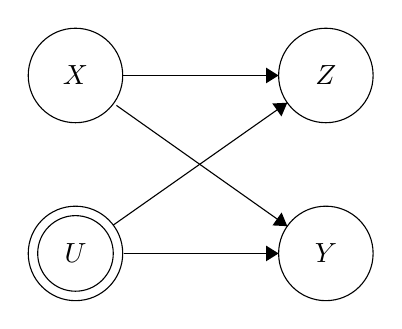
\begin{tikzpicture}[scale=0.2]
\tikzstyle{every node}+=[inner sep=0pt]
\draw [black] (21.5,-21.3) circle (3);
\draw (21.5,-21.3) node {$X$};
\draw [black] (37.4,-21.3) circle (3);
\draw (37.4,-21.3) node {$Z$};
\draw [black] (37.4,-32.6) circle (3);
\draw (37.4,-32.6) node {$Y$};
\draw [black] (21.5,-32.6) circle (3);
\draw (21.5,-32.6) node {$U$};
\draw [black] (21.5,-32.6) circle (2.4);
\draw [black] (24.5,-21.3) -- (34.4,-21.3);
\fill [black] (34.4,-21.3) -- (33.6,-20.8) -- (33.6,-21.8);
\draw [black] (24.1,-23.2) -- (34.95,-30.87);
\fill [black] (34.95,-30.87) -- (34.59,-30) -- (34.01,-30.82);
\draw [black] (23.9,-30.8) -- (34.95,-23.03);
\fill [black] (34.95,-23.03) -- (34,-23.08) -- (34.58,-23.9);
\draw [black] (24.6,-32.6) -- (34.4,-32.6);
\fill [black] (34.4,-32.6) -- (33.6,-32.1) -- (33.6,-33.1);
\end{tikzpicture}
\end{center}

\textit{Example Nominal Propensity Score:}
$e_n(x) = P(Z = 1 | Morning Sickness = Yes)$\\\\
In this case, even if $X \perp Z | Y(0), Y(1)$, $e_n(x)$ is not sufficient for ignorability due to the unobserved confounding factor U. Therefore, adjusting for propensity scores may not remove all the bias in estimating the treatment effect.

\subsection{More on Propensity Scores}

\subsubsection{A Dimension Reduction Perspective on Propensity Scores}
From the dimension reduction viewpoint, propensity scores help simplify the dimensional problem of covariate adjustment by condensing multiple high-dimensional covariates into a single propensity score — the probability of receiving the treatment given the covariates X. The theorem below reduces the dimension of covariates while maintaining ignorability.
\\\\
\textbf{Theorem:}
\begin{center}
    If $Z \perp (Y(1), Y(0)) \thinspace|\thinspace X$
then $Z \perp (Y(1), Y(0)) \thinspace|\thinspace e(X)$
\end{center}

\subsubsection{Propensity Score Stratification}
We now introduce a method for estimating causal effect called Propensity Score Stratification.
\begin{enumerate}
    \item Estimate propensity score by regressing $Z \sim X \rightarrow \hat{e}(x)$
    \item Discretize $\hat{e}(x)$ into k quantities $\rightarrow \hat{e}'(x) = e_k$
    \item Analyze as SRE (Stratified Random Experiment)
\end{enumerate}

We see that $Z \perp (Y(1), Y(0)) \thinspace|\thinspace \hat{e}'(x) = e_k$ approximately holds for $k = 1,2,...,k$\\\\
Empirically, it often appears that getting the correct ordering of propensity scores is more important than obtaining the exact values. The reason lies in how propensity scores are used in practice: their primary function is to balance covariates between treatment and control groups. This balancing typically relies more on the relative ranking of the propensity scores than their precise numerical values.


\textbf{Key Questions:}
\begin{enumerate}
    \item How to choose k?
    \begin{itemize}
        \item If k is too small, then ignorability will be violated
        \item If k is too large, then we cannot analyze as SRE
        \item In 1985, Rosenbaum and Rubin published a widely regarded paper that recommended to use $k=5$
        \item We can increase k as long as each stratum has enough control and treated units
        \item We can decide k after looking at X and Z, however, we should fix k before looking at the outcome Y
    \end{itemize}
    \item How to estimate standard errors when propensity score is estimated?
    \begin{enumerate}
        \item \underline{Use SRE as a conservative estimate}; The estimate is conservative because estimated propensity scores decrease asymptotic variance for estimating causal effect.
        \item \underline{Bootstrap (include propensity score estimation)}; This theory is unclear due to discreteness of the estimator.
    \end{enumerate}
\end{enumerate}

\subsubsection{A Covariate Balancing Perspective on Propensity Scores}
The covariate balancing perspective focuses on the role of propensity scores in balancing covariates between treated and untreated groups. The idea is that once individuals are matched or stratified based on their propensity scores, the distribution of covariates should be similar between the two groups, as would be the case in a randomized controlled trial.

$$ Z \perp X | e(X)$$

\begin{itemize}
    \item Within the same level of $e(x)$, covariate distributions are balanced in expectation across treatment and control
    \item In practice, we can check for covariate balance as a check on how good two propensity score model is
\end{itemize}

\textbf{When to use propensity score models vs. outcome models?}
\begin{enumerate}
    \item Depends on how well you think you can estimate one vs. the other
    \item Do both and see if their causal estimates align:
    \begin{itemize}
        \item If their causal estimates differ, this suggests misspecification
        \item If estimates align, maybe we got the right causal estimate...
    \end{itemize}
    \item Can we combine the propensity score model estimates and outcome regression estimate to get a better estimate of the causal effect?
\end{enumerate}

\subsection{Doubly-robust Estimators}
Doubly-robust estimators are also known as:
\begin{enumerate}
    \item Bias-corrected plugin estimators (\emph{plugin} is the other word for \emph{outcome regression})
    \item Model-assisted Horvitz-Thompson estimators \emph{or} Model-assisted IPW estimators
    \item Semi-parametric estimators \emph{or} Semi-parametric efficient estimators
    \item Augmented IPW (AIPW)
    \item Double machine learning estimators
    \item Debiased machine learning estimators
    \item Orthogonal machine learning estimators
\end{enumerate}

\subsubsection{Introducing $\hat{\tau}_{\text{DR}}$}
Recall the formulas for the \textbf{IPW estimator} and the \textbf{outcome regression estimator} are:
\begin{equation}
\hat{\tau}_{\text{IPW}} = \frac{1}{n} \sum_{i=1}^{n} \frac{Z_i \cdot Y_i}{\hat{e}(X_i)} - \frac{1}{n}\sum_{i=1}^{n}\frac{(1-Z_i) \cdot Y_i}{1 - \hat{e}(X_i)}
\end{equation}
\begin{equation}
\hat{\tau}_{\text{Reg}} = \frac{1}{n} \sum_{i=1}^{n} \left( \hat{\mu}_1 \left(X_i\right) - \hat{\mu}_0 \left(X_i\right) \right)
\end{equation}

One of the reasons why we are using the \textbf{outcome regression estimator} is that some of the potential outcomes are missing. Thus we have this formula where each term in the summation is an estimate of the treatment effect for that particular unit. 

However, when we have already observed one potential outcome for every unit, why are we still using the predicted outcomes instead of using whichever we've observed? Again, the observed potential outcome is an observation of the conditional mean. We can reduce variance by directly estimating the conditional mean and plugging in that estimate here. However, we cannot estimate the conditional mean perfectly, so we are trading off the lower variance for a bias in estimation.

Here comes another question: is there really a way that we can use the observed outcomes but still get some nice bias-variance trade-offs? To solve this question, we introduce the \textbf{Doubly-robust estimator} where we use the errors in the estimates of the outcome regression model as a bias correction.

\subsubsection{Formula \& Interpretation}
Formula for the \textbf{Doubly-robust estimator} is:
\begin{equation}
\hat{\tau}_{\text{DR}} = \frac{1}{n} \sum_{i=1}^{n} \{ 
\hat{\mu}_1\left(X_i\right) + \frac{Z_i\left(Y_i - \mu_i\right)}{\hat{e}\left(X_i\right)} - \hat{\mu}_0\left(X_i\right) - \frac{\left(1 - Z_i\right)\left(Y_i - \hat{\mu}_0\left(X_i\right)\right)}{1 - \hat{e}\left(X_i\right)}
\}
\end{equation}

Here we can see that $\hat{\mu}_1\left(X_i\right)$ and $\hat{\mu}_0\left(X_i\right)$ are just the outcome regression estimator. 

The second and fourth terms, $\frac{Z_i\left(Y_i - \mu_i\right)}{\hat{e}\left(X_i\right)}$ and $\frac{\left(1 - Z_i\right)\left(Y_i - \hat{\mu}_0\left(X_i\right)\right)}{1 - \hat{e}\left(X_i\right)}$, display that $Z_i$ are selecting units that received treatments and they are inversely weighing by their propensity score of treatment and control, respectively. 

You can view the two terms as the IPW-weighed, bias-correction terms that are plugged in to reduce the bias of the \textbf{outcome regression model}. This explains why the \textbf{doubly-robust estimator} is also known as the \textbf{bias-corrected plugin estimator}. 

We can also rearrange the terms of the equation $\hat{\tau}_{\text{DR}}$:
\begin{equation}
\hat{\tau}_{\text{DR}} = \frac{1}{n} \sum_{i=1}^{n} \{ 
\frac{Z_i Y_i}{\hat{e}\left(X_i\right)} - \frac{Z_i - \hat{e}\left(X_i\right)}{\hat{e}\left(X_i\right)}\hat{\mu}_1\left(X_i\right) - \frac{\left(1 - Z_i\right) Y_i}{1 - \hat{e}\left(X_i\right)} - \frac{\left(\hat{e}\left(X_i\right) - Z_i\right)}{1 - \hat{e}\left(X_i\right)}\hat{\mu}_0\left(X_i\right)
\}
\end{equation}

where the first and third terms are usual IPW terms. The second and fourth terms here are the \emph{augmentation terms} that are augmenting the IPW by incorporating the outcome regression model estimates. This explains why the \textbf{doubly-robust estimator} is also known as the \textbf{augmented IPW (AIPW) estimator}. 


\textbf{Relationship with Machine Learning}

It's popular to use Machine Learning to estimate functions such as propensity scores, so people refer to $\hat{\tau}_{\text{DR}}$ also as the \textbf{double machine learning} and \textbf{debiased machine learning estimators} (bias-corrected as proved above).





\section{Lecture Nine: Doubly Robust Estimator (cont.)}
{Taejun Lee \& Zach Rewolinski \& Reet Mishra}

\subsection{Doubly Robust Estimator}
From last lecture:

\[\hat{\tau}_{\text{DR}} = \frac{1}{n} \sum\limits_{i=1}^{n} \left\{\hat{\mu}_1(X_i) + \frac{Z_i(Y_i - \hat{\mu}_1(X_i))}{\hat{e}(X_i)} - \hat{\mu}_0(X_i) - \frac{(1 - Z_i)(Y_i - \hat{\mu}_0(X_i))}{1 - \hat{e}(X_i)}\right\}\]

$\hat{\tau}_{DR}$ is flexible, avoids parametric assumptions, and gets confidence intervals. We call the doubly robust estimator ``double machine learning" because we use machine learning to estimate the nuisance functions $e(X)$, $\mu_0(X)$, and $\mu_1(X)$.

\subsubsection{Advantages of Doubly Robust Estimator (in Parametric Setting)}
\begin{itemize}
    \item Robust to misspecification in either $e(X)$ or $(\mu_1(X),\mu_0(X))$ (hence ``doubly robust").
    \item Can quantify confidence intervals on causal effect.
\end{itemize}

\subsubsection{Proof of Robustness to Misspecification}
\[\hat{\tau}_{\text{DR}} = \frac{1}{n} \sum_{i=1}^{n} \left\{\frac{Z_i(Y_i - \hat{\mu}_1(X_i))}{\hat{e}(X_i)} - \frac{(1 - Z_i)(Y_i - \hat{\mu}_0(X_i))}{1 - \hat{e}(X_i)} + \hat{\mu}_1(X_i) - \hat{\mu}_0(X_i)\right\}\]
\[\mathbb{E}\left[\hat{\tau}_{\text{DR}}\right] = \mathbb{E}\left[\frac{Z(Y - \hat{\mu}_1(X))}{\hat{e}(X)} - \frac{(1 - Z)(Y - \hat{\mu}_0(X))}{1 - \hat{e}(X)} + \hat{\mu}_1(X) - \hat{\mu}_0(X)\right]\]

\textbf{Case 1: $\hat{\mu}_1(X) = \mu_1(X)$ and $\hat{\mu}_0(X) = \mu_0(X)$}
\begin{align*}
    \mathbb{E}\left[\hat{\tau}_{\text{DR}}\right] &= \mathbb{E}\left[\frac{Z(Y - \mu_1(X))}{\hat{e}(X)} - \frac{(1 - Z)(Y - \mu_0(X))}{1 - \hat{e}(X)} + \mu_1(X) - \mu_0(X)\right] \\
    &= \mathbb{E}\left[\mathbb{E}\left[\frac{Z(Y - \mu_1(X))}{\hat{e}(X)} - \frac{(1 - Z)(Y - \mu_0(X))}{1 - \hat{e}(X)} + \mu_1(X) - \mu_0(X) \, \middle| \, X, Z\right]\right] \\
    &= \mathbb{E}\left[\frac{Z}{\hat{e}(X)}\mathbb{E}[Y \, | \, X, Z = 1] - \frac{Z}{\hat{e}(X)}\mu_1(X)\right. \\
    &\quad \left. - \left(\frac{1 - Z}{1 - \hat{e}(X)}\mathbb{E}[Y \, | \, X, Z = 0] - \frac{1 - Z}{1 - \hat{e}(X)}\mu_0(X)\right) + \mu_1(X) - \mu_0(X)\right] \\
    &= \mathbb{E}[\mu_1(X) - \mu_0(X)] \\
    &= \tau
\end{align*}

\textbf{Case 2: $\hat{e}(X) = e(X)$}
\begin{align*}
    \mathbb{E}\left[\hat{\tau}_{\text{DR}}\right] &= \mathbb{E}\left[\frac{Z}{\hat{e}(X)}(\mu_1(X) - \hat{\mu}_1(X)) - \frac{(1 - Z)}{1 - \hat{e}(X)}(\mu_0(X) - \hat{\mu}_0(X)) + \hat{\mu}_1(X) - \hat{\mu}_0(X) \, \middle| \, X\right] \\
    &= \mathbb{E}\left[\frac{e(X)}{e(X)}(\mu_1(X) - \hat{\mu}_1(X)) - \frac{1-e(X)}{1-e(X)}(\mu_0(X) - \hat{\mu}_0(X)) + \hat{\mu}_1(X) - \hat{\mu}_0(X)\right] \\
    &= \mathbb{E}[\mu_1(X) - \mu_0(X)] \\
    &= \tau
\end{align*}

\underline{\textbf{Theorem: $\hat{\tau}_{\text{DR}} - \mathbb{E}[\hat{\tau}_{\text{DR}}] = 0$ if 1) $\hat{e}(X) = e(X)$ OR 2) $\hat{\mu}_1(X) = \mu_1(X)$ and $\hat{\mu}_0(X) = \mu_0(X)$}}

\subsubsection{A Few Perspectives on the Doubly Robust Estimator}

\begin{enumerate}
    \item Reduces the bias of the outcome regression estimator.

    Assume estimand is $\mathbb{E}[Y(1)]$. Then we have $\hat{\tau}_{reg}^1=\frac{1}{n}\sum_{i=1}^n\hat{\mu}_1(X_i)$, which has a bias of $\mathbb{E}\left[\hat{\tau}^1_{reg}-Y(1)\right]=\mathbb{E}\left[\hat{\mu}_1(X)-Y(1)\right]$. Notice that we cannot calculate this quantity because we cannot observe the potential outcomes. Thus, we instead do the following estimate of bias:

    \[\mathbb{E}\left[\frac{Z(\hat{\mu}_1(X)-Y)}{\hat{e}(X)}\right]=B.\]

    The resulting de-biased estimator is \[\frac{1}{n}\sum\limits_{i=1}^n\hat{\mu}_1(X_i)-\frac{1}{n}\sum\limits_{i=1}^n\frac{Z_i(\hat{\mu}_1(X_i)-Y_i)}{\hat{e}(X_i)}.\]

    \item Reduces the variance of the IPW estimator.

    Recall that \[\tau_{IPW}=\frac{1}{n}\sum\limits_{i=1}^n\frac{Z_iY_i}{\hat{e}(X_i)}-\frac{(1-Z_i)Y_i}{1-\hat{e}(X_i)}\] can have high variance because we may be dividing by something which is close to zero.

    Instead, we can divide the residual term by $\hat{e}(X_i)$ so that it blows up less in the event that $\hat{e}(X_i)$ is close to zero or one:

    \[\hat{\tau}^1_{DR}=\frac{1}{n}\sum\limits_{i=1}^n\frac{Z_i(Y_i-\hat{\mu}_1(X_i))}{\hat{e}(X_i)}+\hat{\mu}_1(X).\]
\end{enumerate}

\subsubsection{Confidence Intervals}

\begin{enumerate}
    \item Nonparametric bootstrap
    \item Wald-type normal approximation under certain conditions:
    \begin{itemize}
        \item Sample-splitting: We use one half of the sample to estimate $e(X), \mu_0(X), \mu_1(X)$ and use the other half to estimate $\hat{\tau}_{DR}$ given $\hat{e}(X), \hat{\mu}_0(X), \hat{\mu}_1(X)$. Repeat the process starting with the second half to estimate the nuisance functions and average the results.
        \item Flexible nonparametric methods to estimate nuisance functions $e(X), \mu_0(X), \mu_1(X)$.
    \end{itemize}
    $\hat{\tau}_{DR} - \hat{\tau}$ is asymptotically normal with variance $\frac{var(\phi(X,Y,Z))}{n}$ where

    \[\phi(X,Y,Z)=\frac{Z}{e(X)}(Y-\mu_1(X))-\frac{(1-Z)}{1-e(X)}(Y-\mu_0(X))+\mu_1(X)-\mu_0(X).\]
    
\end{enumerate}

Caution: doubly fragile in a parametric setting

Bias: $\hat{\tau}^1_{DR}-\mathbb{E}[Y(1)]=\mathbb{E}\left[\frac{e(X)-\hat{e(X)}}{e(X)}(\mu_1(X)-\hat{\mu}_1(X))\right]$

Kang \& Schafer (2005) showed this product can make errors large when both $\hat{e}(X)$ and $\hat{\mu}_1(X)$ are misspecified.

\subsection{Causal Estimands Beyond $E[Y(1) - Y(0)]$}

Another estimand of interest is $\tau_T=\mathbb{E}[Y(1)-Y(0)|Z=1]$
\begin{itemize}
    \item ``Average causal effect on the treated".
    \item Allows us to learn about effects of removing an exposure.
    \item Relevant when its infeasible to assign treatment to everyone.
    \begin{itemize}
        \item Example: lottery to attend magnet school.
        \item Example: invasive surgery for high-risk patients
    \end{itemize}
    \item Advantage: requires weaker identifying assumptions.
\end{itemize}

We now need to identify $\tau_T$, specifically the term in \textcolor{red}{red} below:

\[\tau_T=\mathbb{E}[Y\mid Z=1]-\textcolor{red}{\mathbb{E}[Y(0)\mid Z=1]}.\]

Assumptions:
\begin{itemize}
    \item One-sided ignorability: $Z\perp Y(0)\mid X$.
    \item One-sided positivity: $e(X)<1$.
\end{itemize}

\subsubsection{Theorem}

Under one-sided ignorability and positivity,
\begin{enumerate}
    \item $\tau_T=\mathbb{E}[Y\mid Z=1]-\mathbb{E}\left[\mathbb{E}[Y\mid Z=0,X]\mid Z=1\right]$
    \item $\tau_T=\mathbb{E}[Y\mid Z=1]-\mathbb{E}\left[\frac{e(X)}{P(Z=1)}*\frac{(1-Z)Y}{1-e(X)}\right]$
\end{enumerate}

\subsubsection{Proof of Theorem 1}

Part 1:

We want to show that $\mathbb{E}[Y\mid Z=1]=\mathbb{E}\left[\mathbb{E}[Y\mid Z=0,X]\mid Z=1\right]$.
\begin{proof}
\begin{align*}
    \mathbb{E}[Y\mid Z=1]&=\mathbb{E}\left[\mathbb{E}[Y(0)\mid Z=1,X]\mid Z=1\right]\\
    &=\mathbb{E}\left[\mathbb{E}[Y(0)\mid Z=0,X]\mid Z=1\right]\\
    &=\mathbb{E}\left[\mathbb{E}[Y\mid Z=0,X]\mid Z=1\right]\\
\end{align*}
\end{proof}

END OF LECTURE.


\section{Lecture Ten: Matching in Observational Studies}
{Nikhil Shanbhag \& Boyu Fan \& Yichen Xu}

\subsection{Estimator for Average Causal Effect on the Treated}

\subsubsection{Assumptions}

\begin{itemize}
    \item One-sided ignorability: $Z \perp Y(0) | X$
    \item One-sided positivity: $P(e(X) > 0) = 1$
\end{itemize}

\subsubsection{Definition}

Define estimator for the average causal effect on the treated group to be $$\tau_{T} = \mathbb{E}[Y(1) - Y(0) \mid Z = 1] = E[Y \mid Z = 1] - E[Y \mid Z = 0].$$

\subsubsection{Theorem}

$$\tau_T = \mathbb{E}[Y \mid Z = 1] - \mathbb{E}[\mathbb{E}[Y \mid Z = 0, X] \mid Z = 1] = \mathbb{E}[Y \mid Z = 1] - \mathbb{E}\left[\frac{e(X)}{P(Z=1)} \cdot \frac{(1-Z)}{(1-e(X))} Y \mid Z = 1\right].$$

\subsubsection{Proof}

One-sided ignorability implies $Y(0) \perp Z \mid X$ and one-sided positivity implies $P(e(X) > 1) = 1.$

\noindent To show the first line of the theorem, $$\mathbb{E}[Y(0) \mid Z = 1] = \mathbb{E}[\mathbb{E}[Y(0) \mid Z = 1, X] \mid Z = 1] = $$
$$\mathbb{E}[\mathbb{E}[Y(0) \mid Z = 0, X] \mid Z = 1] = \mathbb{E}[\mathbb{E}[Y \mid Z = 0, X] \mid Z = 1].$$

\noindent Notice we can condition on $X$ to rewrite: 
$$\mathbb{E}\left[\frac{ZY(0)}{e}\right] = \frac{\mathbb{E}\left[\mathbb{E}[ZY(0) \mid X]\right]}{e} = \frac{\mathbb{E}\left[\mathbb{E}[Z \mid X]\mathbb{E}[Y(0) \mid X]\right]}{e} = \frac{\mathbb{E}\left[e(X)\mathbb{E}[Y(0) \mid X]\right]}{e}.$$

\noindent The RHS can be written as $$\mathbb{E}\left[\frac{e(X)}{e} \cdot \frac{(1-Z)Y}{1-e(X)} \mid X\right] = \mathbb{E}\left[\frac{e(X)}{e} \cdot \frac{\mathbb{E}[(1-Z)Y \mid X]}{1-e(X)}\right] = \mathbb{E}\left[\frac{e(X)}{e} \mathbb{E}[Y \mid Z=0, X]\right] = $$

$$\mathbb{E}\left[\frac{e(X)}{e} \mathbb{E}[Y(0) \mid X]\right]$$ by using the Tower property. This completes the proof. 

\subsection{Regression estimator}

\subsubsection{Definition}

Consider $$\tau_T = \mathbb{E}[Y \mid Z = 1] - \mathbb{E}[\mathbb{E}[Y \mid Z = 0, X] \mid Z = 1].$$

Define $$\hat{\tau}_T^{\text{reg}} = \frac{1}{n_1} \sum_{i=1}^{n} Y_i Z_i - \frac{1}{n_1} \sum_{i=1}^{n} Z_i \hat{\mu}_0(X_i),$$ where $\hat{\mu}_0(X)$ is the outcome model for $E[Y|Z=0,X]$ learned by regressing $Y \sim X \mid Z=0.$

In order to compute $$\frac{1}{n_1} \sum_{i=1}^{n} Z_i \left(Y_i - \hat{\mu}_0(X_i)\right),$$ recall the IPW estimators and specifically the 2nd identification, which is $$\tau_{T} = E[Y \mid Z=1] = \mathbb{E}\left[\frac{e(X)}{e} \cdot \frac{(1-Z)Y}{1-e(X)}\right].$$ 

\subsubsection{Derivation of Other Estimators}
\noindent This allows us to derive three estimators: (1) Horvitz-Thompson, (2) Hajek, and (3) Odds Ratio. They can written as follows: 

$$\hat{\tau}_T^{\text{ht}} = \frac{1}{n_1} \sum_{i=1}^{n} Z_i Y_i - \frac{1}{n_1} \sum_{i=1}^{n} \frac{\hat{e}(X_i)(1-Z_i) Y_i}{1 - \hat{e}(X_i)}$$

$$\hat{\tau}^{\text{Hajek}} = \frac{1}{n_1} \sum_{i=1}^{n} Z_i Y_i - \frac{\sum_{i=1}^{n} \frac{\hat{e}(X_i)(1-Z_i)Y_i}{1 - \hat{e}(X_i)}}{\sum_{i=1}^{n} \frac{\hat{e}(X_i)(1-Z_i)}{1 - \hat{e}(X_i)}}$$

$$\tau^{\text{OR}} = \frac{1}{n} \sum_{i=1}^{n} Z_i Y_i + \text{DR}(\mathbb{E}[Y(0) \mid Z = 1]) = \frac{1}{n_1} \sum_{i=1}^{n} \left\{ \frac{\hat{e}(X_i)}{1 - \hat{e}(X_i)} (1 - Z_i)(Y_i - \hat{\mu}_0(X_i)) + Z_i \hat{\mu}_0(X_i) \right\},$$ where DR represents the doubly robust estimator.

\subsubsection{Theorem}

Under one-sided ignorability and overlap, if either $\hat{e}(X) = e(X)$ or $\hat{\mu_0}(X) = \mu_0(X)$, then this estimator is unbiased.

\subsubsection{Proof}

The following is an alternative way to rewrite the doubly robust estimator: $$\hat{\tau}_T^{\text{DR}} = \hat{\tau}_T^{\text{Reg}} - \frac{1}{n_1} \sum_{i=1}^{n} \left[\frac{\hat{e}(X_i)}{1 - \hat{e}(X_i)} (1-Z_i)(Y_i - \hat{\mu}_0(X_i))\right] = \hat{\tau}_T^{\text{ht}} - \frac{1}{n_1} \sum_{i=1}^{n} \left[\frac{\hat{e}(X_i)}{1 - \hat{e}(X_i)} (1-Z_i) Z_i \right]\hat{\mu}_0(X_i).$$

The causal effect on the overlap population is then determined by the estimand 
$$\tau_0 = \frac{\mathbb{E}[e(X)(1-e(X))\tau(X)]}{\mathbb{E}[e(X)(1-e(X))]},$$ where $\tau(X)$ represents largest weights for units with $e(X) = \frac{1}{2}.$

Recall: 
$$\tau = \mathbb{E}[Y(1) - Y(0)]$$
$$\tau_{T} = \mathbb{E}[Y(1)-Y(0) \mid Z=1]$$
$$\tau_0 = \frac{\mathbb{E}[e(X)(1-e(X))\tau(X)]}{\mathbb{E}[e(X)(1-e(X))]}.$$

\subsection{Heterogeneous Causal Effects and Effect Modification}

\subsubsection{Definitions}

Let $V$ be a covariate, e.g., male/female. The heterogeneous causal effect is defined as:
\[
\tau_{HCE} = \mathbb{E}[Y(1) - Y(0) | V = v]
\]

A covariate $V$ is called an \emph{effect modifier} if:
\[
\mathbb{E}[Y(1) - Y(0) | V = v] \neq \mathbb{E}[Y(1) - Y(0)]
\]
and $V$ is not affected by the treatment $Z$. If $V$ is affected by treatment, this would instead be called a mediator.

The value of $\tau_{HCE}$ depends on the causal estimand.

\subsubsection{Example}

\[
P(Y(0) = 1 | V = 1) = 0.8
\]
\[
P(Y(1) = 1 | V = 1) = 0.9
\]
\[
P(Y(0) = 1 | V = 0) = 0.1
\]
\[
P(Y(1) = 1 | V = 0) = 0.2
\]

The heterogeneous causal effect is:
\[
\tau_{HCE} = 0.1
\]

Now consider:
\[
\frac{P(Y(1) = 1 | V = 1)}{P(Y(0) = 1 | V = 1)} = \frac{0.9}{0.8} = \frac{9}{8}
\]
\[
\frac{P(Y(1) = 1 | V = 0)}{P(Y(0) = 1 | V = 0)} = 2
\]

We have ``effect measure modifier" and ``effect heterogeneity"

\subsubsection{Why Do We Care?}

\begin{enumerate}
    \item $\tau$ could be zero, but $\tau_{HCE} \neq 0$, meaning the effect differs for different subpopulations.
    \item We want to identify who benefits from the treatment.
\end{enumerate}

\subsubsection{Examples}

\paragraph{Moving to Opportunity (MTO) Experiment:} A randomized experiment gave vouchers to families in public housing to move to richer neighborhoods. One outcome was mental health. The results showed that mental health improved for females but not for males, indicating an effect modification based on gender.

\paragraph{Direct Cash Transfers in Kenya:} The effect of cash transfers on reducing childhood mortality was particularly strong for families who gave birth during the program. This suggests targeting families accordingly in future interventions. Additionally, the overall effect could be muted in geographies with fewer people of child-bearing age.

Effect modifiers are also referred to as \emph{effect-measure modifiers} or \emph{effect heterogeneity}.

\subsubsection{Definition}

Transportability refers to the extrapolation of causal effects computed in one population to a second. Lack of transportability corresponds to a lack of external validity.

\subsubsection{Example: Transportability Issue}

An example where transportability was questioned is the study by Smith and Pell (2003), which found no effect modifiers for the effect of parachutes on high-altitude jumping, showing that the reduction in death after a jump may not be generalizable across populations or situations.

\subsection{RCT vs. Observational Studies}

\subsubsection{Randomized Controlled Trials (RCT)}

\textbf{Advantages:}
\begin{itemize}
    \item High confidence in causal effect for a particular context.
\end{itemize}

\textbf{Disadvantages:}
\begin{itemize}
    \item Expensive to scale.
\end{itemize}

\subsubsection{Observational Studies}

\textbf{Advantages:}
\begin{itemize}
    \item Easy to scale.
    \item Allows investigation across different contexts.
\end{itemize}

\textbf{Disadvantages:}
\begin{itemize}
    \item Make strong assumptions.
\end{itemize}

END OF LECTURE.



\section{Lecture Eleven: Matching in Observational Studies \& Causal DAGs}{Grace Yin \& Haodong Ling \& Zhengxing Cheng}

\subsection{Last Time:}
- RCT shows conflicting results. So the solution is using a meta-analysis of RCTs and observational studies clarified that certain outcomes, like pulmonary embolism, increased under HRT, while others, such as myocardial infarction, decreased.


\subsection{Matching in Observational Studies}
\begin{itemize}
    \item \textbf{Goal}: Construct a subset of the population in which covariates have the same distribution in the treated and control groups.
    \item Intuitive and interpretable.
\end{itemize}

\subsubsection{Matching with Many More Control Units}

%\subsubsection{Ideal Settings}
\begin{center}
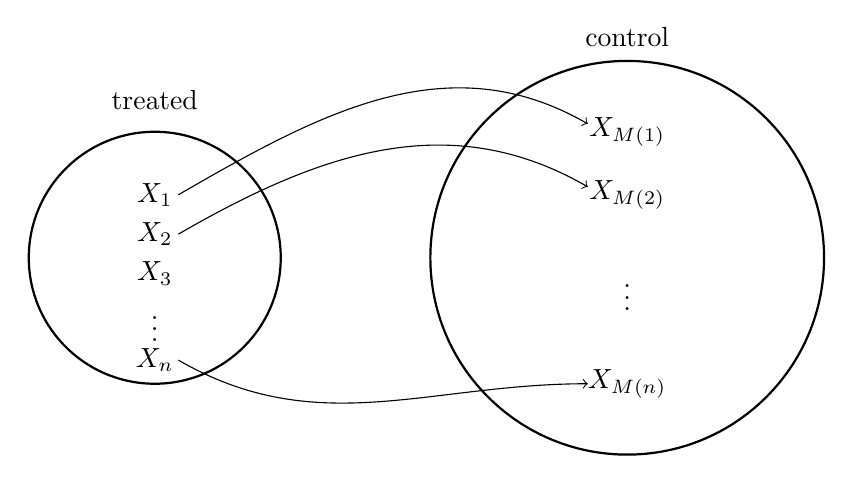
\begin{tikzpicture}

% Circles for treated and control groups
\draw[thick] (-3,0) circle [radius=1.6]; % treated group
\draw[thick] (3,0) circle [radius=2.5]; % control group

% Labels for treated group
\node at (-3,2) {treated};
\node at (-3,0.8) {$X_1$};
\node at (-3,0.3) {$X_2$};
\node at (-3,-0.2) {$X_3$};
\node at (-3,-0.8) {$\vdots$};
\node at (-3,-1.3) {$X_n$};

% Labels for control group
\node at (3,2.8) {control};
\node at (3,1.6) {$X_{M(1)}$};
\node at (3,0.8) {$X_{M(2)}$};
\node at (3,-0.4) {$\vdots$};
\node at (3,-1.6) {$X_{M(n)}$};

% Matching lines
\draw[->] (-2.7,0.8) to[out=30,in=150] (2.5,1.7); % X1 to Xm(1)
\draw[->] (-2.7,0.3) to[out=30,in=150] (2.5,0.9); % X2 to Xm(2)
\draw[->] (-2.7,-1.3) to[out=-30,in=180] (2.5,-1.6); % Xn to Xm(n)

\end{tikzpicture}
\end{center}

where $X_i$ is matched to $X_{M(i)}$.

\begin{itemize}
\item \textbf{Ideal Settings:} we would find exact matches: $X_i = X_{M(i)} \Rightarrow e(X_i) = e(X_{M(i)})$.
    \begin{itemize}
        \item Matches pair experiment assuming $Y(0), Y(1) \perp Z | X$.
        \item Positivity holds in matching by construction.
    \end{itemize}
\item \textbf{More Realistic Settings: Imperfect Matching }
    \begin{itemize}
    \item Almost always the case in observational studies because the covariate space can be large (e.g., continuous features).
    \[
    m(i) = \arg \min_{k: Z_k = 0} d(X_i, X_k)
\]
where $d(X_i, X_k)$ is a distance metric.
    \end{itemize}
\end{itemize}

%\subsubsection{Realistic Settings: Imperfect Matching}
%\begin{itemize}
%    \item Ideally, we would find exact matches: $X_i = X_{m(i)} \Rightarrow e(X_i) = e(X_{m(i)})$.
%    \item Matched pair experiment assuming $Y(0), Y(1) \perp Z \mid X$.
%    \item Positivity holds in matching by construction.
%    \item More realistic settings involve \textbf{imperfect matching}:
 %   \begin{itemize}
 %       \item Almost always the case in observational studies because the covariate space can be large (e.g., continuous features).
 %   \end{itemize}
%end{itemize}

\subsubsection{Distance Metrics for Matching}
 Two Distance Metrics examples are:
\begin{itemize}
    \item \textbf{Euclidean}: 
    \[
    d(X_i, X_k) = (X_i - X_k)^\top (X_i - X_k)
    \]
    \item \textbf{Mahalanobis}: 
    \[
    d(X_i, X_k) = (X_i - X_k)^\top \Sigma^{-1} (X_i - X_k)
    \]
    where $\Sigma$ is the sample covariance matrix of $X$'s in the population.
    \begin{itemize}
        \item Accounts for differences in scale across covariates and correlations between them.
    \end{itemize}
\end{itemize}

\subsubsection{Covariate Adjustment}
Additionally, use covariate adjustment in analysis to correct for the residual covariate imbalance.

\subsubsection{Handling High-Dimensional Covariates}
\textbf{Problem}: When $X$ is high-dimensional, for some $X_i$, $\min\limits_{k: Z_k = 0} d(X_i, X_k)$ is too large.

\textbf{Solutions}: 

\begin{enumerate}
    \item Discard these $X_i$'s:
    \begin{itemize}
        \item Effectively changes the study population.
    \end{itemize}
    \item Dimension reduction before matching:
    \begin{itemize}
        \item e.g., Propensity score matching.
        \item $m(i) = \arg \min\limits_{k: Z_k = 0} |\hat{e}(X_i) - \hat{e}(X_{m(i)})|$
    \end{itemize}
\end{enumerate}


\subsubsection{Algorithm for Matching Multiple Control Units for Treated Unit}
Allow for $M_i$ Control Units for Treated Unit $X_i$:
\begin{itemize}
    \item Input to the matching algorithm: Specify the number of control units, as well as lower or/and upper bounds on $M_i$.

     \item Matching algorithm outputs matched sets, $M_i$ chosen to minimize:
    \[
    \frac{1}{M_i} \sum_{j \in J_i} d(X_i, X_j)
    \]
    where $d(X_i, X_j)$ is a distance function and $J_i$ is the set of indices for control units matched to treated unit $X_i$.
\end{itemize}

\subsubsection{Assessing the Distance Metric}
\begin{itemize}
    \item \textbf{Recap of Ignorability}: $Y(0), Y(1) \perp Z \mid X$ is impossible to empirically verify.
    \item \textbf{How to assess whether the distance metric is good?}
    \begin{itemize}
        \item Analyze covariate distributions in treated vs. matched controls using visualizations like boxplots, or by computing moments of empirical distributions.
    \end{itemize}
\end{itemize}

\subsubsection{Matching Paradigm and Estimand}
\begin{itemize}
    \item Matching paradigm connects to our earlier discussion of the estimand: $\tau_T$ (average causal effect among treated).
    \[
    \tau_T = \mathbb{E}[Y(1) - Y(0) \mid Z = 1] = \mathbb{E}[Y \mid Z = 1] - \mathbb{E}[\mathbb{E}[Y \mid Z = 0, X] \mid Z = 1]
    \]
    \item \textbf{Matching Estimator}:
    \[
    \hat{\tau}_T = \frac{1}{n} \sum_{i=1}^{n} Z_i Y_i - Z_i \hat{\mu}(X_i)
    \]
    where $\hat{\mu}(X_i) = \frac{1}{m_i} \sum_{j \in J_i} Y_j$.

\end{itemize}
This concludes our discussion on matching...

\subsection{Causal DAGs}

From now on, we begin our discussion on Causal Directed Acyclic Graphs (DAGs), which are powerful tools in causal inference. A famous quote, "\textit{Draw your assumptions before your conclusions,}" emphasizes the importance of understanding underlying assumptions in any causal analysis. 

In the computer science (CS) and artificial intelligence (AI) literatures, causal DAGs are extensively used to model relationships between variables. Pioneering work by researchers like Judea Pearl, Peter Spirtes, and Clark Glymour. 

\begin{example}
    Consider the following scenario: $X$, a confounder (e.g., nausea); $Z$, a treatment (e.g., drinking coffee); and $Y$, an outcome (e.g., miscarriage). In the following diagram, the DAG illustrate how the confounder $X$ might influence both the treatment $Z$ and the outcome $Y$. 

\begin{center}
\begin{tikzpicture}
    % Nodes
    \node (X) at (0,0) {$X$};
    \node (Z) at (3,0) {$Z$};
    \node (Y) at (6,0) {$Y$};
    
    % Arrows
    \draw[->] (X) -- (Z);
    \draw[->] (Z) -- (Y);
    \draw[->] (X) to[out=50,in=130] (Y);
    
    % Time arrow
    \draw[->] (-1,-1.5) -- (7,-1.5) node[anchor=north] {time};
\end{tikzpicture}
\end{center}
\end{example}


Here are the meanings of some common notations in causal DAGs:

\begin{itemize}
    \item $V \rightarrow W$ means $V$ has a direct causal effect on $W$ (an effect not mediated by another variable in the graph) for at least one individual.
    \item Lack of an arrow encodes the assumption that there is no direct causal effect of $V$ on $W$ for anyone.
\end{itemize}

Now, let's formally introduce Causal Directed Acyclic Graphs (Causal DAGs), which are essential tools for representing and analyzing causal relationships between variables in a structured, visual manner. Let's break down the key components:

\begin{itemize}
    \item \textbf{Directed}: Causal DAGs include directed arrows between variables to indicate causal effects. For example, $X \rightarrow Z$ means $X$ has a direct causal effect on $Z$.
    \item \textbf{Acyclic}: The graph is acyclic, meaning it cannot contain cycles like $X \rightleftarrows Z$ (where $X$ causes $Z$ and $Z$ causes $X$), as such relationships are not allowed.
\end{itemize}


Some key definitions are listed below:

\begin{definition}[Causal DAG] 
A DAG that satisfies the Causal Markov Assumption.
\end{definition}

\begin{definition}[Causal Markov Assumption] 
Conditional on its direct causes, any variable in a causal DAG is independent of any other variable that it does not cause.
\end{definition}

Causal DAGs represent causal relationships through properly ordered arrows (e.g., $X \rightarrow Y \rightarrow Z$) and associations through improperly ordered arrows (e.g., $X \rightarrow Z \leftarrow Y$).

\subsubsection{Backdoor Path}

A backdoor path is a non-causal path between two variables that can create spurious correlations. Backdoor paths are important because they can make it difficult to determine if an association between two variables is a result of a causal effect or a backdoor path. 

\begin{example}
    $Z$ and $Y$ are linked by a backdoor path, so that are associated. This type of path creates confounding and needs to be accounted for when estimating causal effects.

\begin{center}
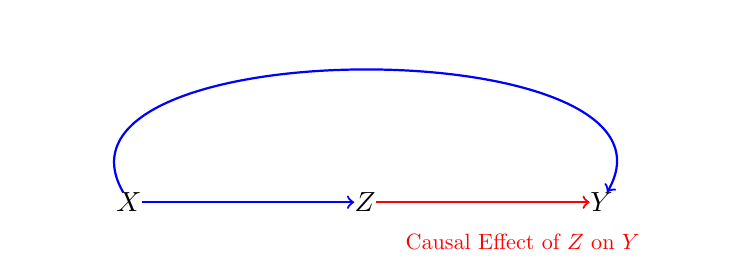
\begin{tikzpicture}

    % Nodes
    \node (X) at (0,0) {$X$};
    \node (Z) at (3,0) {$Z$};
    \node (Y) at (6,0) {$Y$};
    
    % Arrows for the causal diagram
    \draw[->, thick, blue] (X) -- (Z);
    \draw[->, thick, red] (Z) -- (Y) node[midway, below] {};
    \draw[->, thick, blue, out=120, in=60] (X) to (Y);

    % Labels
    \node[red,scale=0.8] at (5, -0.5) {Causal Effect of $Z$ on $Y$};
    
\end{tikzpicture}
\end{center}

\begin{center}
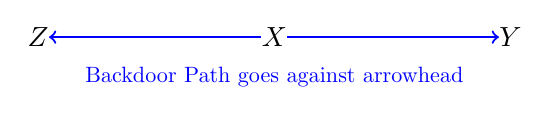
\begin{tikzpicture}

    % Nodes
    \node (Z) at (0,0) {$Z$};
    \node (X) at (3,0) {$X$};
    \node (Y) at (6,0) {$Y$};
    
    % Arrows for the backdoor path (going against arrowhead direction)
    \draw[->, thick, blue] (X) -- (Y);
    \draw[<-, thick, blue] (Z) -- (X);
    

    % Label
    \node[blue, scale=0.8] at (3,-0.5) {Backdoor Path goes against arrowhead};
    
\end{tikzpicture}
\end{center}
\end{example}


\begin{example}
    Suppose variable $Z$ is Carries lighter, $Y$ means Lung cancer, and $X$ means cigarette smoker. $Z$ and $Y$ have an association through $X$ by a backdoor path, but no direct causal effect.

\begin{center}
\begin{tikzpicture}

    % Nodes
    \node (X) at (0,0) {$X$};
    \node (Z) at (3,0) {$Z$};
    \node (Y) at (6,0) {$Y$};
    
    % Arrows for the causal diagram
    \draw[->, thick, black] (X) -- (Z);
    \draw[->, thick, black, out=120, in=60] (X) to (Y);

\end{tikzpicture}
\end{center}
\end{example}

\subsubsection{Colliding}

In causal DAGs, a variable is a collider when it is causally influenced by two or more variables. For example, in the following diagram, $L$ is a collider, as it is causally influenced by $Z$ and $Y$.

\begin{center}
\begin{tikzpicture}
    % Nodes
    \node (Z2) at (0,0) {$Z$};
    \node (Y2) at (3,0) {$Y$};
    \node (L) at (6,0) {$L$};
    
    % Arrows for association through a shared effect

    \draw[->] (Y2) -- (L);
    
    % Curve from Z to L
    \draw[->] (Z2) .. controls (1.5,1.5) and (4.5,1.5) .. (L);
\end{tikzpicture}
\end{center}

\begin{definition} [collider]
Common effect is a \textbf{collider}.
\end{definition}

\begin{definition}
    Graphical structure of a collider is a \textbf{V-structure}, shown in the diagram below.
\end{definition} 

\begin{center}
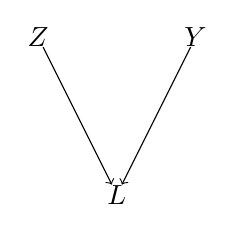
\begin{tikzpicture}
    % Nodes
    \node (Z) at (0,2) {$Z$};
    \node (Y) at (2,2) {$Y$};
    \node (L) at (1,0) {$L$};
    
    % Arrows for the V-structure
    \draw[->] (Z) -- (L);
    \draw[->] (Y) -- (L);
\end{tikzpicture}
\end{center}

In the V-structure, we have:
\begin{itemize}
    \item No association unconditionally between $Z$ and $Y$: $Z \perp\!\!\!\perp Y$
    \item $Z$ and $Y$ are not independent when conditioning on $L$: $Z \not\!\perp\!\!\!\perp Y \mid L$
\end{itemize}

\begin{example}
    Consider $Z$ means poor time management, $Y$ means family emergency and $L$ means missed class. The relationship of $Z$, $Y$ and $L$ are shown as the V-structure, then $Z \perp\!\!\!\perp Y$. However, if I know that a student missed class, then if you tell me whether the student has poor time management skills, it is relevant for my guess about a family emergency occurring.  This phenomenon is what we called  \textit{"explaining away"}.
\end{example}

\subsubsection{Dependency in Causal DAGs}

Now we introduce how we represent conditioning in causal DAGs. 

\begin{example}
    Consider the following diagram. Suppose $Z$ means taking aspirin, $M$ means platelet aggregation and $Y$ means heart disease, 
\begin{center}
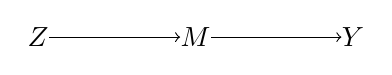
\begin{tikzpicture}
    % Nodes
    \node (Z) at (0,0) {$Z$};
    \node (M) at (2,0) {$M$};
    \node (Y) at (4,0) {$Y$};
    
    % Arrows for causal pathway
    \draw[->] (Z) -- (M);
    \draw[->] (M) -- (Y);
\end{tikzpicture}
\end{center}
Is there an association between $Z$ and $Y$ within levels of $M$ (e.g., conditional on $M$)? To study this question, we use the following diagram, where the box around $M$ indicates conditioning on $M$.

\begin{center}
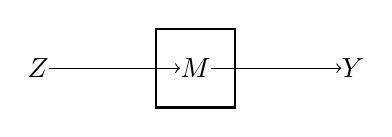
\begin{tikzpicture}
    % Nodes
    \node (Z2) at (0,0) {$Z$};
    \node (M2) at (2,0) {$M$};
    \node (Y2) at (4,0) {$Y$};
    
    % Arrows for blocked pathway
    \draw[->] (Z2) -- (M2);
    \draw[->] (M2) -- (Y2);
    
    % Box around M to indicate conditioning
    \draw[thick] (1.5,-0.5) rectangle (2.5,0.5);
\end{tikzpicture}
\end{center}

\end{example}


\section{Lecture 12: Paths of association and d-separation}{James Bowden}

\subsection{Last Time: Causal DAG definitions}

\begin{example}
    Consider the following diagram. Suppose \( Z \): taking aspirin, \( M \): platelet aggregation, and \( Y \): heart disease.
\begin{center}
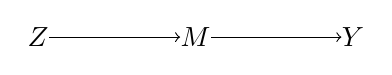
\begin{tikzpicture}
    % Nodes
    \node (Z) at (0,0) {$Z$};
    \node (M) at (2,0) {$M$};
    \node (Y) at (4,0) {$Y$};
    
    % Arrows for causal pathway
    \draw[->] (Z) -- (M);
    \draw[->] (M) -- (Y);
\end{tikzpicture}
\end{center}
Is there an association between \( Z \) and \( Y \) when conditioned on \( M \)? To study this question, we use the following diagram, where the box around $M$ indicates conditioning on $M$.

\begin{center}
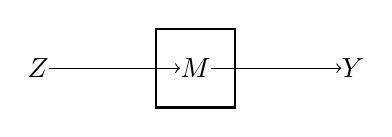
\begin{tikzpicture}
    % Nodes
    \node (Z2) at (0,0) {$Z$};
    \node (M2) at (2,0) {$M$};
    \node (Y2) at (4,0) {$Y$};
    
    % Arrows for blocked pathway
    \draw[->] (Z2) -- (M2);
    \draw[->] (M2) -- (Y2);
    
    % Box around M to indicate conditioning
    \draw[thick] (1.5,-0.5) rectangle (2.5,0.5);
\end{tikzpicture}
\end{center}
\end{example}

New objects introduced in the context of causal graphs include confounders, backdoor paths (non-causal), colliders (variables causally influenced by two or more variables), and mediators (which yield causal independence when conditioned upon).


\subsection{Revisiting common cause structure}

\begin{example}
In this diagram, there's a direct causal path, $Z\rightarrow Y$, and an associative path, $Z \leftarrow X \rightarrow Y$. $X$ is called a \textbf{confounder}.

\begin{center}
\begin{tikzpicture}
    % Nodes
    \node (X) at (0,0) {$X$};
    \node (Z) at (3,0) {$Z$};
    \node (Y) at (6,0) {$Y$};
    
    % Arrows
    \draw[->] (X) -- (Z);
    \draw[->] (Z) -- (Y);
    \draw[->] (X) to[out=50,in=130] (Y);
    
\end{tikzpicture}
\end{center}

We can also denote blocking the associative path with a box, meaning $Z \perp Y(z) | X$. In this case, $X$ no longer confounds the relationship between $Z$ and $Y$; that is, we will only observe how changes in $Z$ not induced by $X$ affect $Y$.

\begin{center}
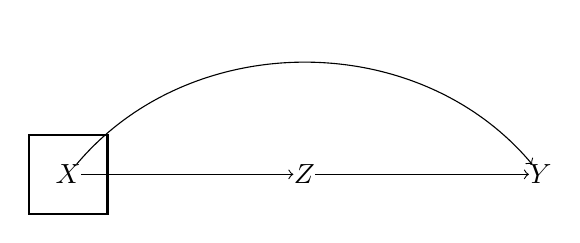
\begin{tikzpicture}

    % Nodes
    \node (X) at (0,0) {$X$};
    \node (Z) at (3,0) {$Z$};
    \node (Y) at (6,0) {$Y$};
    
    % Arrows
    \draw[->] (X) -- (Z);
    \draw[->] (Z) -- (Y);
    \draw[->] (X) to[out=50,in=130] (Y);
    
    % Box around X to indicate conditioning
    \draw[thick] (-0.5,-0.5) rectangle (0.5,0.5);
\end{tikzpicture}
\end{center}
\end{example}

\subsection{Common effect structure}

\begin{example}
Consider the following causal DAG: $L$ is wet grass, $Z$ is sprinklers ran overnight, $Y$ is that it rained.

\begin{center}
\begin{tikzpicture}
    % Nodes
    \node (Z) at (-1,1) {$Z$};
    \node (Y) at (3,1) {$Y$};
    \node (L) at (1,0) {$L$};
    
    % Arrows for the V-structure
    \draw[->] (Z) -- (L);
    \draw[->] (Y) -- (L);
\end{tikzpicture}
\end{center}
\end{example}

Here, $Z \perp Y$ but $Z \not\perp Y | L$. $L$ is called a \textbf{collider}. Paths of association do not flow through colliders (i.e., $Z \perp Y$). However, if we were to condition on $L$ (or some descendent thereof), denoted in a causal DAG as a box around $L$, then association would flow through $L$ (i.e., $Z \not\perp Y | L$). This is because when $L$ has been fixed as a known quantity, knowing something about $Z$ will provide information about $Y$ (and vice versa). One can see this through the simple relationship $Z+Y=L$ where $Z \perp Y$ but if $L$ is known, then knowing $Z$ yields $Y$ as $Y=L-Z$.

\subsection{Recap}
\subsubsection{Why might 2 variables be associated? Structural reasons:}

\begin{enumerate}
\item One causes the other
\item The two share a common cause (a confounder)
\item The two share a common effect, and our analysis looks at a certain level that effect (i.e., conditional on a value of $L=l$ in the diagram immediately above).
\end{enumerate}

\subsubsection{A causal DAG implies a set of structural equations}

\begin{center}
\begin{tikzpicture}
    % Nodes
    \node (X) at (0,0) {$X$};
    \node (Z) at (3,0) {$Z$};
    \node (Y) at (6,0) {$Y$};
    
    % Arrows
    \draw[->] (X) -- (Z);
    \draw[->] (Z) -- (Y);
    \draw[->] (X) to[out=50,in=130] (Y);
    
\end{tikzpicture}
\end{center}

What equations does this graph imply?
\begin{itemize}
\item $X \sim F_X(X)$
\item $Z \sim g_Z(X, \epsilon_Z)$
\item $Y \sim g_Y(X, Z, \epsilon_Y)$
\end{itemize}

\subsection{Exchangeability}

\subsubsection{Causal graphs + exchangeability}

If we know the true causal DAG, then we can determine whether there exists a set of variables $X$ s.t. $Z \perp Y(1), Y(0) | X$. This leads us to the backdoor criterion.

\begin{definition}[Backdoor criterion]
The backdoor criterion holds for a set of covariates $X$ when all backdoor paths (non-causal associative paths) between $Z$ and $Y$ are blocked by conditioning on $X$, and $X$ contains no variables that are descendents of $Z$. The backdoor criterion implies exchangeability conditional on $X$. 
\end{definition}

\begin{example}
In the below DAG, there is a backdoor path through $X$.
\begin{center}
\begin{tikzpicture}
    % Nodes
    \node (X) at (0,0) {$X$};
    \node (Z) at (3,0) {$Z$};
    \node (Y) at (6,0) {$Y$};
    
    \node (L) at (3,-1) {$L$};
    
    % Arrows
    \draw[->] (X) -- (Z);
    \draw[->] (Z) -- (Y);
    \draw[->] (X) to[out=50,in=130] (Y);
    \draw[->] (L) -- (Y);
    
\end{tikzpicture}
\end{center}

In order to make the backdoor criterion hold, we must condition on $X$, denoted by a box: 

\begin{center}
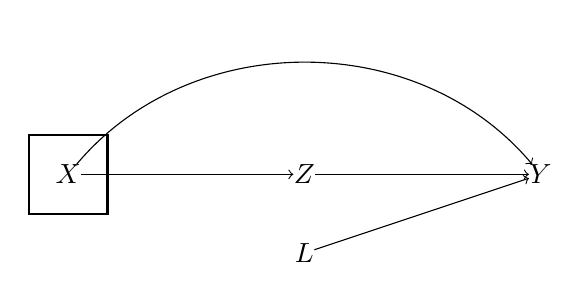
\begin{tikzpicture}
    % Nodes
    \node (X) at (0,0) {$X$};
    \node (Z) at (3,0) {$Z$};
    \node (Y) at (6,0) {$Y$};
    
    \node (L) at (3,-1) {$L$};
    
    % Arrows
    \draw[->] (X) -- (Z);
    \draw[->] (Z) -- (Y);
    \draw[->] (X) to[out=50,in=130] (Y);
    \draw[->] (L) -- (Y);

    % Box around X to indicate conditioning
    \draw[thick] (-0.5,-0.5) rectangle (0.5,0.5);
    
\end{tikzpicture}
\end{center}

Now there are no backdoor paths, so the backdoor criterion is fulfilled. 
\end{example}

\begin{example}
Let $Z$ be aspirin, $Y$ is stroke, and $X$ is doctor diagnosis of previous underlying health conditions.

\begin{center}
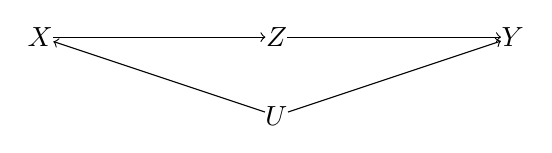
\begin{tikzpicture}
    % Nodes
    \node (X) at (0,0) {$X$};
    \node (Z) at (3,0) {$Z$};
    \node (Y) at (6,0) {$Y$};
    
    \node (U) at (3,-1) {$U$};
    
    % Arrows
    \draw[->] (X) -- (Z);
    \draw[->] (Z) -- (Y);
    % \draw[->] (X) to[out=50,in=130] (Y);
    \draw[->] (U) -- (Y);
    \draw[->] (U) -- (X);
    
\end{tikzpicture}
\end{center}

What paths go from $Z$ to $Y$? There's the direct causal path $Z \rightarrow Y$ as well as a backdoor path, $Z \leftarrow X \leftarrow U \rightarrow Y$. 
As such, $U$ is a \textbf{common cause}. 

To fulfill the backdoor criterion, we can block the backdoor path in two different ways: via conditioning on either $U$ or $X$.

\begin{center}
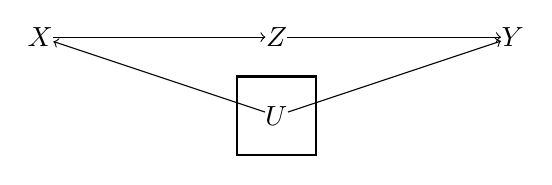
\begin{tikzpicture}
    % Nodes
    \node (X) at (0,0) {$X$};
    \node (Z) at (3,0) {$Z$};
    \node (Y) at (6,0) {$Y$};
    
    \node (U) at (3,-1) {$U$};
    
    % Arrows
    \draw[->] (X) -- (Z);
    \draw[->] (Z) -- (Y);
    % \draw[->] (X) to[out=50,in=130] (Y);
    \draw[->] (U) -- (Y);
    \draw[->] (U) -- (X);

    % Box around X to indicate conditioning
    \draw[thick] (2.5,-1.5) rectangle (3.5,-0.5);
    
\end{tikzpicture}
\end{center}

\begin{center}
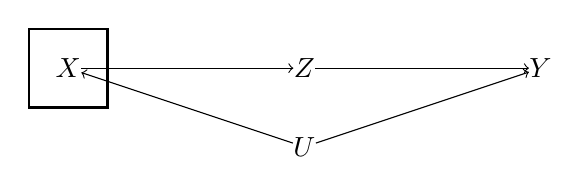
\begin{tikzpicture}
    % Nodes
    \node (X) at (0,0) {$X$};
    \node (Z) at (3,0) {$Z$};
    \node (Y) at (6,0) {$Y$};
    
    \node (U) at (3,-1) {$U$};
    
    % Arrows
    \draw[->] (X) -- (Z);
    \draw[->] (Z) -- (Y);
    % \draw[->] (X) to[out=50,in=130] (Y);
    \draw[->] (U) -- (Y);
    \draw[->] (U) -- (X);

    % Box around X to indicate conditioning
    \draw[thick] (-0.5,-0.5) rectangle (0.5,0.5);
    
\end{tikzpicture}
\end{center}
\end{example}

\subsubsection{Recap}
Causal graphs are useful for thinking about confounding because:
\begin{itemize}
    \item We make assumptions about the data generating process explicit.
    \item They enable us to find the set of confounders (if possible) to achieve exchangeability under those assumptions.
\end{itemize}

\subsubsection{Other methods for assessing exchangeability}

Recall that exchangeability, $Z \perp Y(1), Y(0) | X$ is untestable. This is because it implies
$$P(Y(1)=1|Z=1,X) = P(Y(1)=1|Z=0,X)$$
and while the former term is observable, the latter is the counterfactual and is not ever known. \textit{Note that we can write the analogous equation for $Y(0)$ and observe the same issue}. 

As such, we cannot ever test this assumption formally. We can, however, assess the strength of evidence in support of exchangeability to validate (or call into question) our assumption.

\begin{enumerate}
    \item Use data on other outcomes: "negative outcomes".
    
    Suppose we observe $\Tilde{Y}$. Assume:
    \begin{itemize}
        \item The confounding of $\Tilde{Y}$ is the same as the confounding for $Y$ w.r.t. $Z$
        \item $Z$ has no effect on $\Tilde{Y}$
    \end{itemize}
    \begin{center}
    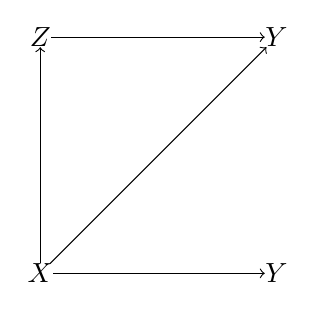
\begin{tikzpicture}
        % Nodes
        \node (X) at (0,0) {$X$};
        \node (Yt) at (3,0) {$\Tilde{Y}$};
        \node (Z) at (0,3) {$Z$};
        \node (Y) at (3,3) {$Y$};
        
        % Arrows
        \draw[->] (X) -- (Z);
        \draw[->] (X) -- (Yt);
        \draw[->] (X) -- (Y);
        \draw[->] (Z) -- (Y);
        
    \end{tikzpicture}
    \end{center}
    In terms of potential outcomes, we would write:
    \begin{itemize}
        \item $Z \perp Y(Z) | X$ and $Z \perp \Tilde{Y(Z)} | X$
        \item $\mathbb{E}[\Tilde{Y}|Z=1]-\mathbb{E}[\Tilde{Y}|Z=0] \neq 0$ if we have confounding 
    \end{itemize}
    \begin{example}
        From Cornfield (1959): $Y$ is lung cancer, $Z$ is cigarette smoking, $\Tilde{Y}$ is car accidents. 

        He found evidence that $\mathbb{E}[\Tilde{Y}|Z=1] = \mathbb{E}[\Tilde{Y}|Z=0]$.

        To the extent that there are common confounders for car accidents and lung cancer, then this supports the claim that the association between lung cancer and smoking is causal. It is noted that there's no real intuition for why car accidents and lung cancer are related, but this example may be illustrative anyway, as an extreme case.
    \end{example}
    \begin{example}
        From Jackson et al. (year?): Let $Y$ be hospitalization during flu season, $\Tilde{Y}$ hospitalization before flu season, $Z$ getting the flu vaccine.

        They found evidence that $\mathbb{E}[\Tilde{Y}|Z=1] - [\Tilde{Y}|Z=0]$ was very large. From this, we can conclude that there were unmeasured confounders, and that the assumption of exchangeability was violated / not reasonable.
    \end{example}
    \item To be continued...
\end{enumerate}





\section{Lecture 13: Negative Outcomes and Instrumental Variables}{Jean Lee}

\subsection{Last Time}

\begin{itemize}
    \item Negative outcomes were used to assess the exchangeability assumption.
    \item Negative outcomes are also known as negative outcome controls or placebo tests. 
    \end{itemize}
    
\textbf{Recall example:}
\begin{itemize}
    \item \( y \): hospitalization during flu season 
    \item \( \tilde{y} \): hospitalization before flu season
    \item \( z \): vaccine
    
\end{itemize}
$\mathbb{E}[\tilde{Y}|Z=1] - \mathbb{E}[\tilde{Y}|Z=0]$ large: suggests unmeasured confounding


\subsubsection{Another Example: lagged outcomes (Imbens and Rubin, 2015)}
\begin{itemize}
    \item Use outcome right before treatment as a negative outcome
    \item Treatment can't affect something that happened before the treatment
    \item The confounding structure may be similar for lagged outcomes
\end{itemize}
Assume the confounding follows:
\[
\mathbb{E}[Y(0) | Z = 1] - \mathbb{E}[Y(0) | Z = 0] = \mathbb{E}[\tilde{Y} | Z = 1] - \mathbb{E}[\tilde{Y}| Z = 0]
\]
This leads to a difference-in-differences model.

\subsection{Assessing Confounding Using Negative Exposures}
Another method to assess confounding is by using data on other treatments/exposures: "Negative Exposures"
\begin{itemize}
    \item $\tilde{Z}$: treatment/exposure variable that shares the same confounding as \(Z\) w.r.t \(Y\)
\end{itemize}
\begin{center}
  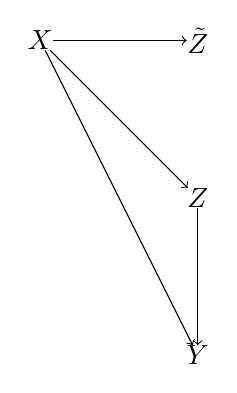
\begin{tikzpicture}
    % Nodes
    \node (X) at (0,0) {$X$};
    \node (Z_tilde) at (2,0) {$\tilde{Z}$};
    \node (Z) at (2,-2) {$Z$};
    \node (Y) at (2,-4) {$Y$};
    
    % Arrows for causal pathway
    \draw[->] (X) -- (Z_tilde);
    \draw[->] (X) -- (Z);
    \draw[->] (Z) -- (Y);
    \draw[->] (X) -- (Y);
\end{tikzpicture}
\end{center}
Assume: $Z \perp\!\!\!\perp Y(Z) \mid X \text{ and } \tilde{Z} \perp\!\!\!\perp Y(Z) \mid X$

\[
\mathbb{E}[Y(\tilde{Z} = 1) - Y(\tilde{Z} = 0)] = 0 
\]

\subsubsection{Example: Sanderson et al 2017}
\begin{itemize}
    \item Let \( Z \) be maternal exposure during pregnancy
    \item Let $\tilde{Z}$ be paternal exposure during pregnancy
    \item Let \( Y \) be the child's BMI or autism spectrum disorder
\end{itemize}

\subsection{Proximal Causal Inference}
Proximal causal inference: when we have both negative outcomes and negative exposures
\begin{itemize}
    \item Conditions under which we can nonparametrically identify the casual effect in the presence of unmeasured confounding 
    \begin{itemize}
    \item Example: 
    
    u: unobserved confounder (discrete)
    
    $\tilde{y}$: negative outcome (discrete)
    
    $\tilde{z}$: negative exposure (discrete)
    \end{itemize}
    \item when $\tilde{y}$ and $\tilde{z}$ have as many levels as u, then we can identify the causal effect
\end{itemize}

\subsection{Colliders and Over-Adjustment Problems}
Recall collider L:
\begin{center}
  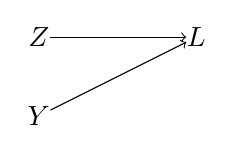
\begin{tikzpicture}
    % Nodes
    \node (Z) at (0,0) {$Z$};
    \node (L) at (2,0) {$L$};
    \node (Y) at (0,-1) {$Y$};
    
    % Arrows for causal pathway
    \draw[->] (Z) -- (L);
    \draw[->] (Y) -- (L);
\end{tikzpicture}
\end{center}
Rule of d-separation: 

$\rightarrow \leftarrow \text{closed}$

$\rightarrow \boxed{L} \leftarrow \quad \text{opens } Z \perp\!\!\!\perp Y \mid L$

\subsubsection{Problem 1: M-Bias}
\textbf{M-bias:}
\begin{center}
  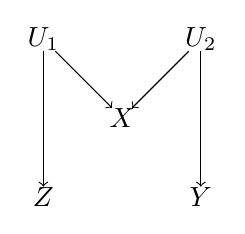
\begin{tikzpicture}
    % Nodes
    \node (U1) at (0,0) {$U_1$};
    \node (U2) at (2,0) {$U_2$};
    \node (X) at (1,-1) {$X$};
    \node (Z) at (0,-2) {$Z$};
    \node (Y) at (2,-2) {$Y$};
    
    % Arrows for causal pathway
    \draw[->] (U1) -- (X);
    \draw[->] (U1) -- (Z);
    \draw[->] (U2) -- (X);
    \draw[->] (U2) -- (Y);
\end{tikzpicture}
\end{center}

\[
\mathbb{E}[Y \mid Z = 1] - \mathbb{E}[Y \mid Z = 0] = 0
\]

\begin{itemize}
    \item valid unbiased estimator for causal effect because there's no confounding
\end{itemize}

If "over-adjust" by condition on X: $Z \perp\!\!\!\perp Y(Z) \mid X$

\[
\mathbb{E}[\mathbb{E}[Y \mid Z=1, X] - \mathbb{E}[Y \mid Z=0, X]] \neq 0
\]

\begin{center}
    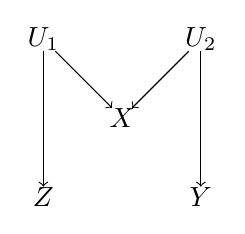
\begin{tikzpicture}
      % Nodes
      \node (U1) at (0,0) {$\boxed{U_1}$};
      \node (U2) at (2,0) {$U_2$};
      \node (X) at (1,-1) {$\boxed{X}$};
      \node (Z) at (0,-2) {$Z$};
      \node (Y) at (2,-2) {$Y$};
      
      % Arrows for causal pathway
      \draw[->] (U1) -- (X);
      \draw[->] (U1) -- (Z);
      \draw[->] (U2) -- (X);
      \draw[->] (U2) -- (Y);
    \end{tikzpicture}%
  \begin{minipage}{0.4\textwidth}
    \centering
    \text{blocks path of association}
  \end{minipage}
\end{center}

\subsubsection{Problem 2: Z-bias}
\textbf{Z-bias:}
\begin{center}
  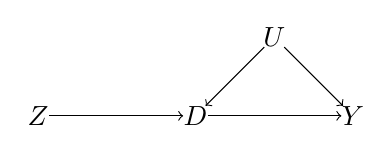
\begin{tikzpicture}
    % Nodes
    \node (Z) at (0,0) {$Z$};
    \node (D) at (2,0) {$D$};
    \node (Y) at (4,0) {$Y$};
    \node (U) at (3,1) {$U$};
    
    % Arrows for causal pathway
    \draw[->] (Z) -- (D);
    \draw[->] (D) -- (Y);
    \draw[->] (U) -- (D);
    \draw[->] (U) -- (Y);
\end{tikzpicture}
\end{center}

\textbf{Key Assumptions:}
\begin{itemize}
\item Instrument Independence: \( Z \perp\!\!\!\perp Y \)
\item Instrument Relevance: \( Z \not\perp\!\!\!\perp D \)
\item Z only affects y through D
\end{itemize}


\begin{itemize}
    \item Generally conditioning on Z will make our estimates more biased
    \begin{itemize}
    \item D: treatment received
    \item Y: outcome
    \item Ch. 16 of A first course example with linear models
    \end{itemize}
    \item Z is not a confounder, but U is and we don't observe U 
    \item Conditioning on Z makes D less random and amplifies the role of U in the remaining randomness of D 
    \item Z: instrumental variable 
    \item Z-bias = instrumental variable bias 
\end{itemize}
Example: 
\begin{itemize}
\item \(D \): prison sentence length 
\item \( Y \) : recommit an offense (re-arrest) after release
\item \( Z \): random assignment of cases to judges 
\item \( U \): personal characteristics, family support
\end{itemize}

What covariates should we adjust for in observational studies?

\begin{center}
  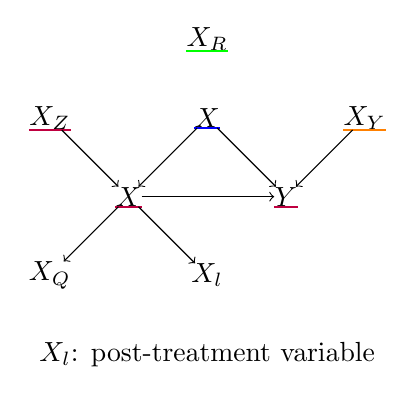
\begin{tikzpicture}
    % Nodes
    \node (XR) at (0,0) {$X_R$};
    \node (XZ) at (-2,-1) {$X_Z$};
    \node (X) at (0,-1) {$X$};
    \node (XY) at (2,-1) {$X_Y$};
    \node (Z) at (-1,-2) {$X$};
    \node (Y) at (1,-2) {$Y$};
    \node (XL) at (0,-3) {$X_l$};
    \node (XQ) at (-2,-3) {$X_Q$};
    \node at (0,-4) {\text{$X_l$: post-treatment variable}}; % Add this line

    % Underline colors
    \draw[green, thick] (XR.south west) -- (XR.south east);
    \draw[purple, thick] (XZ.south west) -- (XZ.south east);
    \draw[blue, thick] (X.south west) -- (X.south east);
    \draw[orange, thick] (XY.south west) -- (XY.south east);
    \draw[purple, thick] (Z.south west) -- (Z.south east);
    \draw[purple, thick] (Y.south west) -- (Y.south east);
    
    % Arrows for causal pathway
    \draw[->] (XZ) -- (Z);
    \draw[->] (X) -- (Z);
    \draw[->] (X) -- (Y);
    \draw[->] (XY) -- (Y);
    \draw[->] (Z) -- (Y);
    \draw[->] (Z) -- (XL);
    \draw[->] (Z) -- (XQ);
\end{tikzpicture}
\end{center}

\begin{center}
\begin{tabular}{|c|c|c|} % Specify three centered columns with borders
\hline
\textbf{Necessary for Identification} & \textbf{Helpful to Reduce Variance} & \textbf{Harmful} \\
\hline
$X$ & $X_Y$ & $X_R$ \\
"confounding" & "effect modifier" & $X_Z$\\
 & & $X_l$\\
\hline
\end{tabular}
\end{center}

\textbf{What to do when it's unreasonable to assume exchangeability}

Today: instrumental variables 

Next week: sensitivity analysis + bounds + partial identification
\subsection{Instrumental Variables}
In experiments, often participants may not adhere/comply to treatment assignment 

\begin{itemize}
    \item \( Z \): treatment assignment
    \item \( D \): the treatment taken, "adherence"
    \item\( U \) : confounders that affect \( Y \) and \( D \)
    \item \( Y \): outcome
\end{itemize}

\begin{center}
  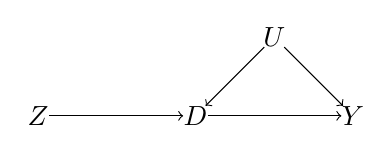
\begin{tikzpicture}
    % Nodes
    \node (Z) at (0,0) {$Z$};
    \node (D) at (2,0) {$D$};
    \node (Y) at (4,0) {$Y$};
    \node (U) at (3,1) {$U$};
    
    % Arrows for causal pathway
    \draw[->] (Z) -- (D);
    \draw[->] (D) -- (Y);
    \draw[->] (U) -- (D);
    \draw[->] (U) -- (Y);
\end{tikzpicture}
\end{center}

\textbf{Example}

\begin{itemize}
    \item
    \begin{itemize}
    \item \( D \): aspirin taken
    \item \( Y \): stroke
    \item \(  Z \): whether patient was assigned aspirin
    \item \( U \): behavioral factors
    \end{itemize}
    \item Challenge: can't measure everything in \( U \)
    \item Solution: leverage randomness in instrument \( Z \)
\end{itemize}

\textbf{Definition:} A \textbf{instrumental variable} is a random variable that meets 3 condition: 
\begin{enumerate}
    \item \tikz[baseline=(X.base)]{
        \node[inner sep=0pt] (X) {\underline{\textbf{Relevance}:}};
        \draw[green, thick] (X.south west) -- (X.south east);
    } $Z \not \perp\!\!\!\perp D$
    \begin{itemize}
    \item \( Z \) is associated with the treatment \( D \)
    \end{itemize}
    \item  \tikz[baseline=(X.base)]{
        \node[inner sep=0pt] (X) {\underline{\textbf{Exclusion Restriction}:}};
        \draw[blue, thick] (X.south west) -- (X.south east);
    }\( Z \) only affects \( Y \) only through \( D \)
    \begin{itemize}
    \item No direct effect of \( Z \) on \( Y \)
    \item e.g., holds double-blind experiment 
    \end{itemize}
 \item \tikz[baseline=(X.base)]{
        \node[inner sep=0pt] (X) {\underline{\textbf{Exchangeable / Unconfounded IV}}}; % Fixed missing closing brace
        \draw[red, thick] (X.south west) -- (X.south east); % Dotted line
    } \( Z \) and \( Y \) don't share unmeasured confounders
\end{enumerate}

\begin{center}
  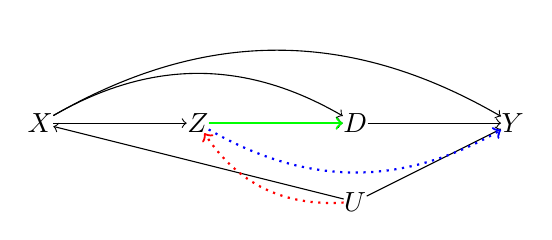
\begin{tikzpicture}
    % Nodes
    \node (X) at (0,0) {$X$};
    \node (Z) at (2,0) {$Z$};
    \node (D) at (4,0) {$D$};
    \node (Y) at (6,0) {$Y$};
    \node (U) at (4,-1) {$U$};
    
    % Arrows for causal pathway
    \draw[->] (X) -- (Z);
    \draw[->] (X) to[bend left] (Y);
    \draw[->] (Z) -- (D);
    \draw[->,  green, thick] (Z) -- (D);
    \draw[->] (D) -- (Y);
    \draw[->] (X) to[bend left] (D);
    \draw[->] (U) -- (X);
    \draw[->] (U) -- (Y);
    \draw[ -> , dotted, blue, thick] (Z) to[bend right] (Y);
    \draw[ -> , dotted, red, thick] (U) to[bend left] (Z);
\end{tikzpicture}
\end{center}
* dotted arrow: not an edge

\textbf{Example:} Minneapolis Domestic Violence Experiment (1980s)

\begin{itemize}
\item randomly assigned penalties:
\begin{enumerate}
\item arrest (1/3)
\item counseling (1/3)
\item separation (1/3)

(arrest, counseling, separation are all \( D \))
\end{enumerate}
\item \( Y \) : re-offense
\item Officers did not always comply
\end{itemize}







